\documentclass[twoside,a4paper,12pt,openany]{book}

\usepackage[latin1]{inputenc}
\usepackage[spanish]{babel}
\usepackage{geometry}
\usepackage{makeidx}
\usepackage{graphicx}
\usepackage{subfig}
\usepackage[Bjornstrup]{fncychap}
\usepackage{a4wide}
\usepackage{named}
\usepackage[table]{xcolor}
\usepackage{listings}
\usepackage{pdfpages}
\usepackage{appendix}
%\DeclareGraphicsExtensions{.jpg,.pdf,.png,.ps}

\usepackage{color}
\definecolor{gray97}{gray}{.97}
\definecolor{gray75}{gray}{.75}
\definecolor{gray45}{gray}{.45}

\pagestyle{headings}
\geometry{a4paper, left=3.5cm, right=2cm, top=3cm, bottom=2cm, headsep=1.5cm}

\widowpenalty=10000
\clubpenalty=10000
\hyphenpenalty=10000
\tolerance=10000
%Para que no corte las palabras al final de la linea.

% Latex command para crear listas sin espacio entre
% un item y otro.
\newenvironment{packed_item}{
\begin{itemize}
  \setlength{\itemsep}{1pt}
  \setlength{\parskip}{0pt}
  \setlength{\parsep}{0pt}
}{\end{itemize}}

% Latex command para crear listas umeradas sin 
% espacio entre un item y otro.
\newenvironment{packed_enum}{
\begin{enumerate}
  \setlength{\itemsep}{1pt}
  \setlength{\parskip}{0pt}
  \setlength{\parsep}{0pt}
}{\end{enumerate}}

% Configuracion del entorno lstlistings
\lstset{ frame=Ltb,
framerule=0pt,
aboveskip=0.5cm,
xleftmargin=0.7cm,
framextopmargin=3pt,
framexbottommargin=3pt,
framexleftmargin=0.4cm,
framesep=0pt,
rulesep=.4pt,
backgroundcolor=\color{gray97},
rulesepcolor=\color{black},
%
stringstyle=\ttfamily,
showstringspaces = false,
basicstyle=\small\ttfamily,
commentstyle=\color{gray45},
keywordstyle=\bfseries,
%
numbers=left,
numbersep=15pt,
numberstyle=\tiny,
numberfirstline = false,
breaklines=true,
}

% minimizar fragmentado de listados
\lstnewenvironment{listing}[1][]
{\lstset{#1}\pagebreak[0]}{\pagebreak[0]}

\lstdefinestyle{consola}
{basicstyle=\scriptsize\bf\ttfamily,
backgroundcolor=\color{gray75},
}

\lstdefinestyle{C}
{language=C,
}

\lstdefinestyle{sh}
{language=sh,
}

\makeindex

\begin{document}

\thispagestyle{empty}

\baselineskip 1.35\baselineskip

\vspace{2cm}

\begin{figure}[htb]
  \centerline{\resizebox{.60\textwidth}{!}{
\includegraphics{img/logo_urjc}}}
\end{figure}

\begin{center}
  {\Large {\bf INGENIER�A EN INFORM�TICA}}
  \vspace{5mm}
 
  {\large {Escuela T�cnica Superior de Ingenier�a Inform�tica}}
  \vspace{5mm}

  {\large {Curso acad�mico 2011/2012}}

  \vspace{1cm}

  {\large {\bf Proyecto Fin de Carrera}}

  \vspace{2cm}

  {\Large {Uso de robots en terapias de Alzheimer\\[1cm] }}

  \vspace{5cm}
  {\bf Autor}: Gonzalo Jos� Abella Dago\\
  {\bf Tutor}: Francisco Mart�n Rico 
\end{center}

\clearpage
\newpage{\pagestyle{empty}\cleardoublepage}
\thispagestyle{empty}

\vspace{5cm}
\makebox[15cm][r]{
  \begin{tabular}{ll}
  \emph{A mi familia, a Emma y a mi padrino.}
  \end{tabular} 
}

\clearpage
\newpage{\pagestyle{empty}\cleardoublepage}
\thispagestyle{empty}

\vspace{5cm}
\textbf{\huge{Agradecimentos}}\\

Quiero agradecer a todos los participantes de este proyecto, que no son pocos, la ayuda prestada y el buen ambiente que hemos tenido: a los investigadores y terapeutas de la Fundaci�n CIEN, a los miembros y profesores del grupo de Rob�tica de la universidad y a todo aquel que ha colaborado con la investigaci�n.\\

En especial quiero dar las gracias a Emma y a mi familia por haberme apoyado y estar siempre ah�. A mi padrino I�igo por animarme a seguir con la carrera en los momentos m�s cr�ticos. Y por �ltimo, a mi tutor Francisco Mart�n por el trabajo y esfuerzo que me ha dedicado durante todo el proyecto.\\

A todos, ��muchas gracias!!
\clearpage
\newpage{\pagestyle{empty}\cleardoublepage}

%%%%%%%%%% RESUMEN %%%%%%%%
\newpage{\pagestyle{empty}\cleardoublepage} 
\vspace{5 cm}
\textbf{\Huge{Resumen}}
\vspace{1.5 cm}

La rob�tica social es un campo de la rob�tica muy atractivo e interesante a cuya investigaci�n la comunidad rob�tica dedica cada vez m�s tiempo, esfuerzo y dinero. La interacci�n hombre-m�quina adquiere un valor esencial en este tipo de robots para que la comunicaci�n entre ambos sea intuitiva. En particular, la rob�tica asistencial se centra en c�mo pueden ayudar los robots a mejorar la calidad de vida de personas discapacitadas o enfermas. Una enfermedad que cada d�a afecta a m�s gente y se invierten m�s recursos en investigar sobre ella, es la enfermedad de Alzheimer.\\

El objetivo de este proyecto es emplear robots en terapias para enfermos de Alzheimer que sean eficaces y f�ciles de usar para el terapeuta. Para ellos hemos creado una aplicaci�n gr�fica que facilita este cometido. Esta herramienta, adem�s de una interfaz gr�fica, permite teleoperar al robot por medio un control remoto externo: el Wiimote.\\

El desarrollo de esta investigaci�n engloba, adem�s de la codificaci�n de la aplicaci�n, todos los aspectos relacionados con el uso y evaluaci�n de un robot en terapias de Alzheimer, y todas las herramientas utilizadas.\\

Esta investigaci�n ha sido realizada en el grupo Grupo de Rob�tica de la Universidad Rey Juan Carlos y se ha hecho en conjunto con un centro de investigaci�n especializado en enfermedades neurol�gicas, la Fundaci�n CIEN.

                                %\pagenumbering{roman}

                                %\setcounter{page}{1}
\frontmatter
\tableofcontents

\listoffigures
                                %\setcounter{page}{1}
                                %\pagenumbering{arabic}
\listoftables

\mainmatter

% Init counter page
\setcounter{page}{1}

% Capitulo 1
\chapter{Introducci�n}
\label{cap:introduccion}

La Rob�tica es uno de los retos tecnol�gicos m�s desafiantes a los que nos enfrentamos. Uno de los objetivos del grupo de Rob�tica de la Universidad Rey Juan Carlos es crear m�quinas que nos hagan la vida m�s f�cil e interact�en con nosotros con cierto grado de autonom�a.\\

Una de las l�neas de investigaci�n del grupo se realiza mediante la participaci�n en la liga de f�tbol de la \textit{RoboCup}\footnote{http://www.robocup.org}, una competici�n que plantea el f�tbol como un banco de pruebas de tecnolog�a rob�tica en la que los robots se enfrentan jugando partidos de f�tbol de manera aut�noma. La \textit{RoboCup} es un proyecto internacional nacido en 1997 y creado para promover, a trav�s de distintas competiciones, la investigaci�n y educaci�n en Inteligencia Artificial y la Rob�tica. En concreto, el grupo participa en la \textit{Standard Platform League}. Esta competici�n se caracteriza por que todos los equipos compiten con el mismo robot, focalizando los esfuerzos en la creaci�n de software. Actualmente se utiliza el humanoide Nao, fabricado por la empresa francesa \textit{Aldebaran Robotics}\footnote{http://www.aldebaran-robotics.com}. La figura \ref{fig:robocup} es una imagen tomada en la Robocup German Open 2012, �ltima competici�n en la que particip� el equipo del grupo de Rob�tica de la Universidad.

\begin{figure} [hbtp]
  \begin{center}
    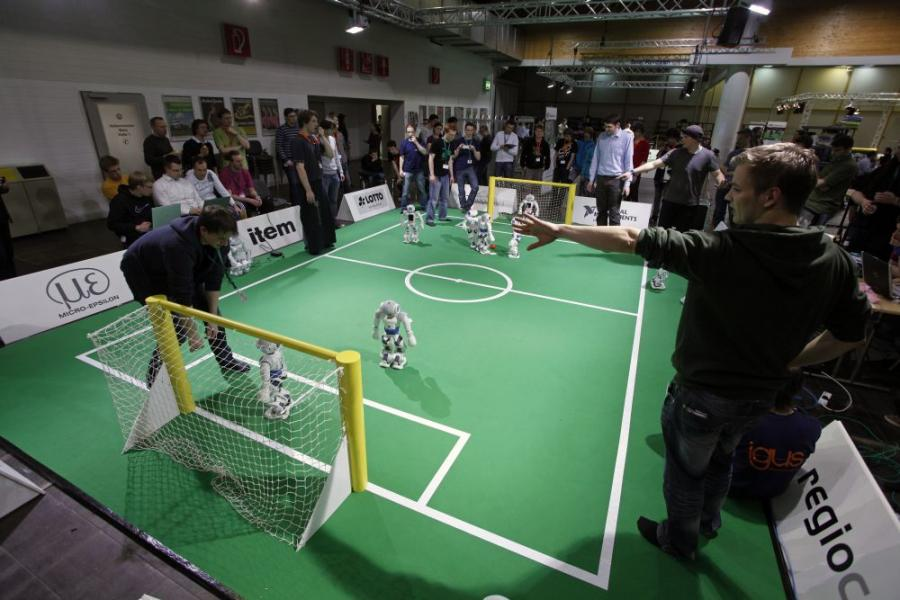
\includegraphics[width=12cm]{img/cap1/robocup}
  \end{center}
  \caption{Imagen de un partido de f�tbol de la Robocup German Open 2012.}
  \label{fig:robocup}
\end{figure}\

Hace tres a�os surgi� la oportunidad, a trav�s de la Fundaci�n CIEN, de poder aplicar todo el software desarrollado para la competici�n en un entorno completamente distinto y con unas metas tambi�n muy diferentes. Se brind� al grupo la posibilidad de aplicar toda esta tecnolog�a rob�tica a un objetivo social empleando los conocimientos adquiridos en la competici�n. Se propuso utilizar al robot como herramienta en una investigaci�n en terapias de la enfermedad de Alzheimer.\\

Este proyecto fin de carrera forma parte de esta investigaci�n, compuesto a su vez por otros proyectos fin de carrera y el trabajo realizado por los miembros del grupo de rob�tica.\\

En este cap�tulo se presenta la rob�tica en t�rminos generales. Se definir� el t�rmino \textit{Robot} y hablaremos de elementos comunes a �stos, independientemente del tipo que sean. Luego se explicar� qu� es la rob�tica m�vil y, por �ltimo, nos centraremos en el �rea de la rob�tica en la que se ubica nuestro proyecto: la rob�tica social. Para terminar se expondr� c�mo est� estructurado este documento.\\

\section{Rob�tica}
\label{sec:robotica}

La rob�tica es la rama de la ciencia que estudia los robots. El t�rmino \textit{Robot} es dif�cil de definir. Fue introducido por el escritor checo Karen Capek en su obra R.U.R. (Robots Universales de Rossum), estrenada en 1921. Esta palabra deriva de la palabra checoslovaca \textit{Robota} que significa literalmente trabajar y figuradamente trabajo duro o penoso. No hay �nica definici�n que satisfaga a todos los organismos internacionales de estandarizaci�n. Por ejemplo, la IFR (International Federation of Robotics) utiliza la definici�n propuesta por la ISO (Organizaci�n Internacional para la Estandarizaci�n) incluido en el ISO 8373. En este documento se define como \textit{manipulador programable en tres o m�s ejes, multiprop�sito, controlado autom�ticamente y reprogramable}. Esta definici�n tambi�n es usada por otros comit�s como el EURON (EUropean RObotics research Network). En cambio, la RIA (Robotic Industries Association) define el t�rmino robot como \textit{manipulador reprogramable y multifuncional dise�ado para mover materiales, partes, herramientas o dispositivos especializados a trav�s de movimientos programados para la realizaci�n de una serie de tareas}. Esta definici�n es un poco m�s amplia que la anterior. Por �ltimo, la RAE define el t�rmino robot como \textit{m�quina o ingenio electr�nico programable, capaz de manipular objetos y realizar operaciones antes reservadas solo a las personas}.\\

Como se puede comprobar, cada una de las definiciones de robot es distinta de las otras. En mi opini�n, la definici�n contenida en la ISO 8373 y la dada por la RIA est�n muy centradas en la rob�tica industrial. De hecho, define al robot como un manipulador. En el lado opuesto, la definici�n proporcionada por la RAE es demasiado amplia y abstracta. A mi juicio, un robot es una m�quina programable capaz de interactuar con su entorno, ya sea modific�ndolo directamente o desplaz�ndose por �l, para realizar una o varias tareas. Las tareas asignadas suelen ser aquellas que por su peligrosidad, repetici�n o precisi�n suponen una liberaci�n para las personas.\\

Desde siempre, el ser humano ha intentado construir m�quinas que le liberen, simplifiquen o faciliten el trabajo. Los antiguos egipcios unieron brazos mec�nicos a las estatuas de sus dioses y los griegos construyeron estatuas con sistemas hidr�ulicos. Estas estatuas automatizadas eran utilizadas para atemorizar, fascinar e infundir respeto al pueblo. Estos inventos pueden considerarse como los primeros \textit{''robots''} de la historia, aunque distan mucho de los robots actuales.\\

El inicio de la rob�tica, tal y como la vemos en estos momentos, puede fijarse en el siglo XVIII. En 1801 el franc�s Joseph Jacquard invent� un telar mec�nico programable mediante tarjetas perforadas (Figura \ref{fig:telar-jacquard-general}). Esta m�quina permit�a elaborar dise�os de telares complejos a usuarios inexpertos. Cada tarjeta perforada correspond�a a una l�nea del dise�o y la uni�n de varias tarjetas formaban un patr�n con el que se tejer�a el telar. En esta �poca tambi�n se construyeron algunos artilugios curiosos, como una mu�eca mec�nica capaz de hacer dibujos de forma aut�noma, inventada por Henri Maillardert, o unos m�sicos de tama�o humano creados por Jacques de Vauncansos. Estos \textit{''robots''} ten�an un prop�sito m�s de ocio que laboral.\\

\begin{figure}[t]
  \centering
  \subfloat[El telar de Jacquard.]{
    \label{fig:telar-jacquard}
    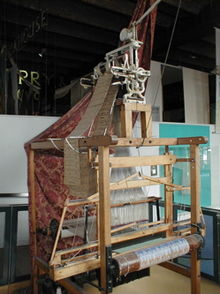
\includegraphics[width=8cm]{img/cap1/telar-jacquard}
  }
  \subfloat[Tarjeta programable del telar.]{
    \label{fig:tarjeta-jacquard}
    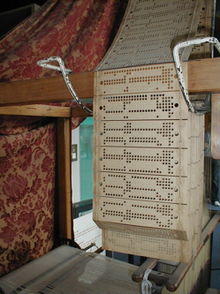
\includegraphics[width=8cm]{img/cap1/tarjeta-jacquard}
  }
  \caption{El telar de Jacquard est� expuesto en el Museo de la ciencia y la industria en Manchester, Inglaterra.}
  \label{fig:telar-jacquard-general}
\end{figure}



Pero no fue hasta mediados del siglo XX, gracias a los avances en inteligencia artificial, cuando se crearon los primeros robots modernos. El primer robot industrial programable se construye e instala en 1961 en la \textit{Ford Motors Company}, se llamaba \textit{Unimate}. Su cometido era el levantar piezas industriales que estaban a altas temperaturas. Sin embargo, es en la d�cada de los 70 cuando comienza a desarrollarse completamente la rob�tica. En 1973 aparece el primer robot con 6 ejes electromec�nicos (Figura \ref{fig:famulus}) y, a los pocos a�os el primer brazo mec�nico programable 
(Figura \ref{fig:puma}). Estos primeros robots modernos eran b�sicamente manipuladores, es decir, brazos mec�nicos fijos en el suelo que realizan una tarea concreta.\\

\begin{figure}[hbtp]
  \centering
  \subfloat[FAMULUS]{
    \label{fig:famulus}
    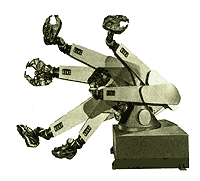
\includegraphics[width=8cm]{img/cap1/famulus}
  }
  \subfloat[PUMA]{
    \label{fig:puma}
    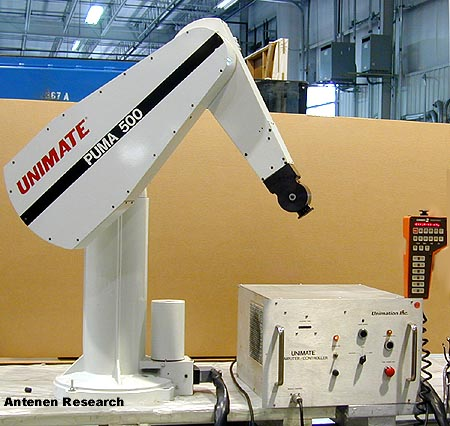
\includegraphics[width=8cm]{img/cap1/puma}
  }
  \caption{Dos de los primeros robots programables en la d�cada de los 70.}
\end{figure}

Los robots definen su funcionalidad y caracter�sticas en funci�n de una serie de elementos hardware. Estos elementos son los encargados de recibir est�mulos, procesarlos y efectuar una respuesta. Los elementos hardware se clasifican en sensores, actuadores y procesadores: 

\begin{itemize}
  \item \textbf{Sensores.} Son dispositivos que miden propiedades del entorno tales como distancia, temperatura, intensidad lum�nica o se�al GPS entre otros. Tambi�n existen los sensores propioceptivos que miden propiedades del robot, como puede ser la temperatura de los motores para prevenir que se quemen o el n�mero de vueltas que da una rueda. Los sensores m�s utilizados son: 
    \begin{enumerate}
      \item \textbf{Ultrasonido.} Es un dispositivo que sirve para medir distancias. La distancia se calcula midiendo el tiempo de vuelo de una onda sonora, cuya frecuencia est� por encima del espectro audible por el o�do humano, emitida por el dispositivo, es decir, el tiempo que tarda la onda en volver despu�s de rebotar en un obst�culo. Una vez conocido el tiempo de vuelo y la velocidad de una onda sonora, la distancia se calcula por medio de una sencilla operaci�n matem�tica. La precisi�n de este dispositivo es bastante pobre.
      \item \textbf{L�ser.} El l�ser tambi�n sirve para medir distancias y �sta se calcula de la misma manera que lo hace el ultrasonido, s�lo que en vez de utilizar una onda sonora, utiliza una frecuencia de luz del espectro no visible. Este dispositivo es m�s preciso que el ultrasonido, pero tambi�n m�s caro. Un ultrasonido tiene un precio del orden de decenas de d�lares, mientras que un l�ser tiene un precio de miles de d�lares.
      \item \textbf{C�mara.} Este sensor es uno de los m�s populares. En un sensor muy rico y barato, el �nico problema de este dispositivo es la dificultad de interpretar las im�genes por el costo computacional que conlleva dicha tarea.
  \end{enumerate}
En la figura \ref{fig:nao-laser} se puede ver al robot Nao equipado con un laser en la cabeza, aunque este dispositivo es opcional. El robot tambi�n dispone de ultrasonidos en el pecho, colocados en la banda azul que rodea el bot�n central, y de dos c�maras colocadas una en la frente y la otra en la boca.

\begin{figure} [hbtp]
  \begin{center}
    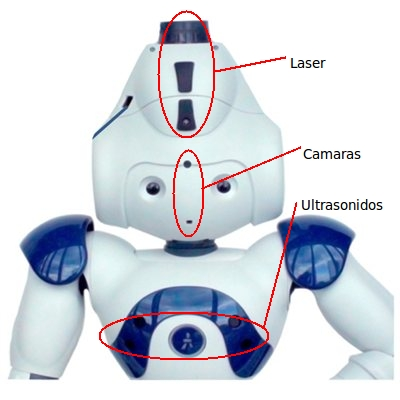
\includegraphics[width=9cm]{img/cap1/nao-laser}
  \end{center}
  \caption{Robot Nao equipado con un laser en la cabeza.}
  \label{fig:nao-laser}
\end{figure}\

\item \textbf{Actuadores.} Son dispositivos que modifican el estado del robot o su entorno. Los manipuladores o brazos rob�ticos son un ejemplo de actuadores que pueden interactuar con el entorno, pero tambi�n lo son los altavoces o los LEDs. Es importante destacar en este punto la existencia de dos grandes familias de robots: los robots fijos y los robots m�viles. Los robots fijos suelen encontrarse en la rob�tica industrial. Los robots m�viles, que como su nombre indica, son aquellos capaces de desplazarse por el entorno. En la siguiente secci�n se hablar� m�s sobre este �ltimo tipo de robot en funci�n de su forma de desplazarse.

\item \textbf{Procesadores.} Son elementos encargados de procesar los datos obtenidos de los sensores, analizarlos, comprenderlos y generar una respuesta que ejecutar�n los actuadores. Comparando un robot con una persona y haciendo una analog�a simple, se puede decir que los sensores, actuadores y procesadores son los sentidos, m�sculos y cerebro, respectivamente.
\end{itemize}


\section{Rob�tica m�vil}
\label{sec:roboticamovil}

Como hemos comentado anteriormente existen dos grandes familias de robots: los robots fijos y los robots m�viles. Los robots fijos son robots que suelen estar anclados al suelo o pueden tener un poco de movimiento por medio de ra�les o alg�n otro m�todo similar que proporcionan al robot una movilidad muy reducida. Los t�picos robots fijos son los manipuladores que se encuentran en las cadenas de montaje. La mayor�a disponen de un brazo mec�nico con varios grados de libertad con el que interact�an con su entorno. Estos robots han evolucionado mucho gracias a la gran inversi�n que ha realizado la industria en las �ltimas d�cadas. En concreto, la industria automovil�stica con la soldadura de carrocer�as ha sido la gran impulsora de la rob�tica industrial.\\

La otra gran familia de robots, los robots m�viles, tambi�n se les conoce como robots de servicio. Este t�rmino, robots de servicio, apareci� a finales de los a�os 80 por la necesidad de construir sistemas y robots que fuesen capaces de trabajar en diferentes entornos, con condiciones ambientales muy diversas y fuesen aut�nomos o pr�cticamente aut�nomos. La caracter�stica principal de este tipo de robots es que pueden desplazarse por el entorno que les rodea para realizar una tarea. Un ejemplo de este tipo de robots es la sonda espacial enviada a Marte por la NASA, Curiosity (Figura \ref{fig:curiosity}). La misi�n de este robot es la de determinar si existi� vida en el planeta y determinar la geolog�a y el clima para estudiar su habitabilidad.

\begin{figure}[hbtp]
  \centering
  \subfloat[Robot soldador]{
    \label{fig:robotsoldador}
    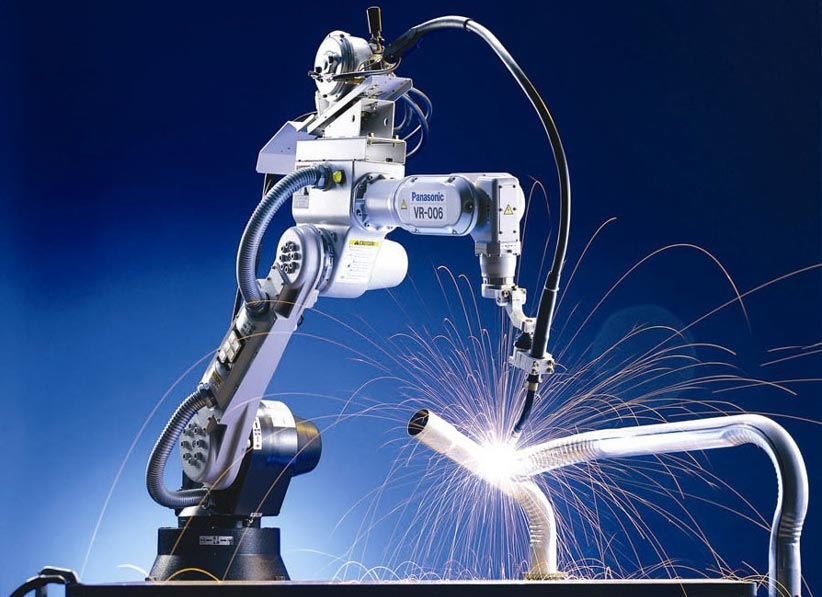
\includegraphics[width=7cm]{img/cap1/robotsoldador}
  }
  \subfloat[Sonda Curiosity]{
    \label{fig:curiosity}
    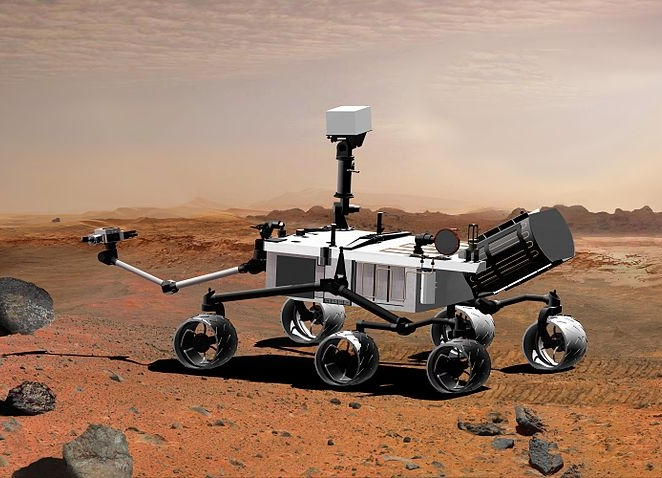
\includegraphics[width=7cm]{img/cap1/curiosity}
  }
  \caption{El robot soldador es un ejemplo de un robot fijo mientras que la sonda Curiosity es un robot m�vil.}
\end{figure}

Los robots m�viles pueden clasificarse seg�n el medio por el que se desplazan porque estos influye de manera determinante en los sensores, los actuadores, la localizaci�n o la navegaci�n. Estos son:

\begin{itemize}
  \item \textbf{Terrestres.} Son los robots m�s comunes y se desplazan por el suelo. Los medios de locomoci�n t�picos son las ruedas y las patas. Las ruedas son los actuadores m�s baratos, sencillos de utilizar y estables. Se pueden conseguir velocidades altas y la odometr�a es bastante precisa. Funcionan muy bien en terrenos llanos o poco abruptos, pero son incapaces de salvar grandes desniveles. La sonda Curiosity (Figura \ref{fig:curiosity}) es un ejemplo de un robot con ruedas.\\
Los robots con patas, en cambio, presenta una serie de dificultades a�adidas que complican su funcionamiento. Primero, es necesario conseguir un buen equilibrio para que el robot sea estable y segundo, coordinar los movimientos de las patas para que �ste se desplace son tareas bastante complejas. Las velocidades que se alcanzan son bajas y la odometr�a es muy imprecisa. A cambio de estos inconvenientes, se gana la capacidad de moverse por mayor diversidad de terrenos, y de construir robots parecidos a animales o a humanos. El robot Aibo (Figura \ref{fig:aibo}) utiliza cuatro patas para desplazarse.\\
Existen otras formas de desplazamiento por el medio terrestre como los robots modulares (Figura \ref{fig:robot-modular}), que imitan el movimientos de las serpientes o de los gusanos para desplazarse.

\begin{figure}[hbtp]
  \centering
  \subfloat[Perrito Aibo]{
    \label{fig:aibo}
    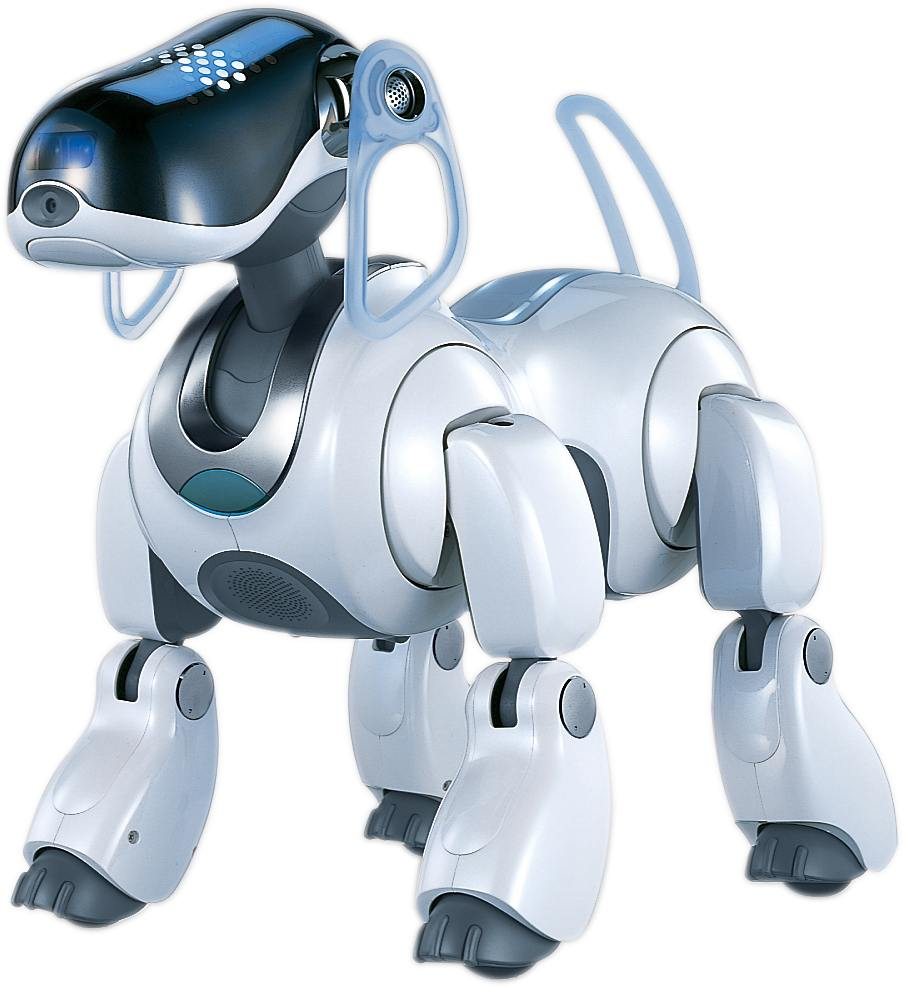
\includegraphics[width=3.5cm]{img/cap1/aibo}
  }
  \subfloat[Robot Pionner equipado con un sensor l�ser]{
    \label{fig:pionner}
    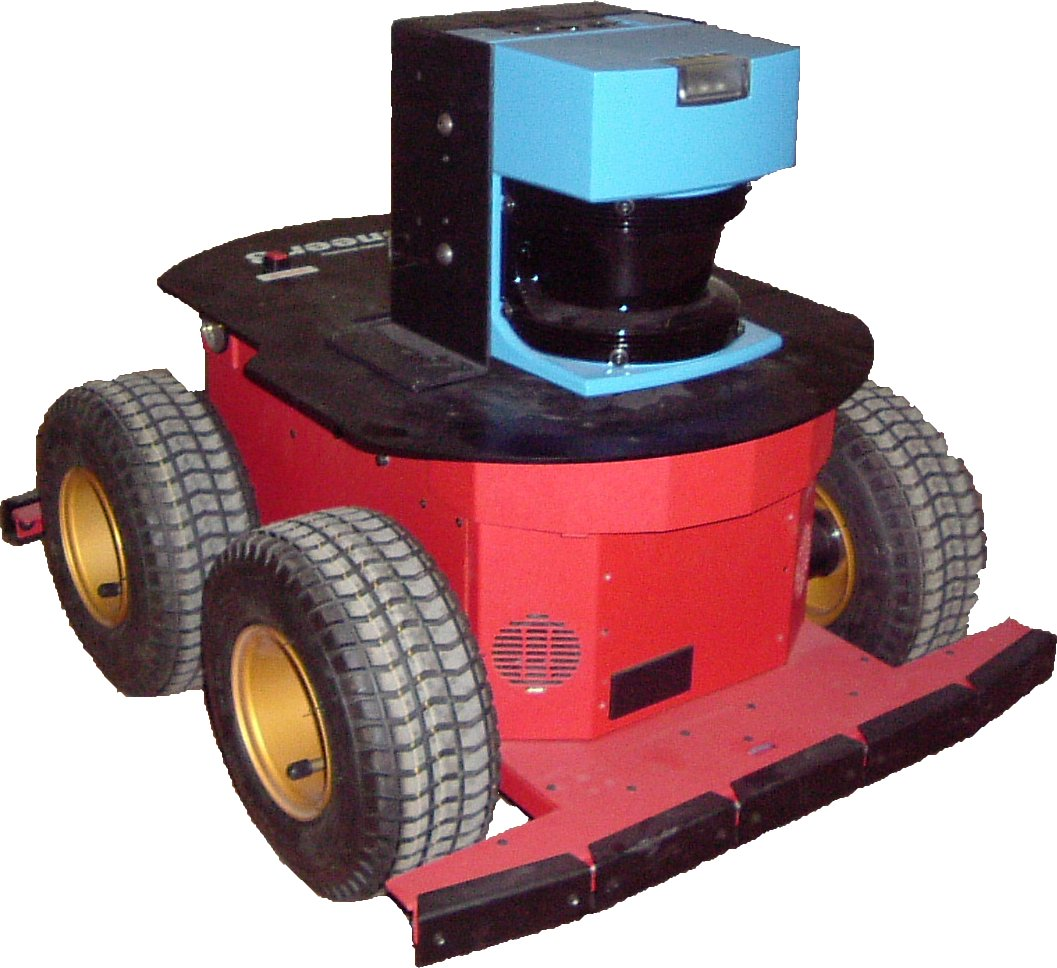
\includegraphics[width=4.5cm]{img/cap1/pionner}
  }
  \subfloat[Robot modular]{
    \label{fig:robot-modular}
    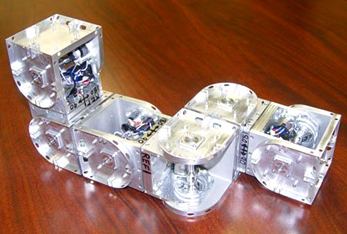
\includegraphics[width=4.5cm]{img/cap1/robot-modular}
  }
  \caption{Distintos ejemplos de robots terrestres.}
\end{figure}

\item \textbf{Voladores.} Los robots voladores son aquellos que se desplazan por el aire. Tambi�n son conocidos por las siglas UAV (\textit{Unmanned Aerial Vehicle)}. Son utilizados mayoritariamente en aplicaciones militares. El m�todo de impulsi�n m�s popular, al igual que en los robots acu�ticos, son las h�lices. Actualmente, se est�n popularizando mucho los cuadric�pteros. Estos robots est�n equipados con cuatro h�lices que le aportan mucha estabilidad y control. En la figura \ref{fig:drone} se puede ver un robot de este tipo, el Parrot AR-Drone. Exceptuando el robot que acabamos de comentar, los UAV son utilizados mayoritariamente en aplicaciones militares. En la figura \ref{fig:avion-espia} tenemos un MQ-9 Reaper. Se trata de una aeronave no tripulada con capacidad de ataque con misiles.

\begin{figure}[hbtp]
  \centering
  \subfloat[MQ-9 Reaper]{
    \label{fig:avion-espia}
    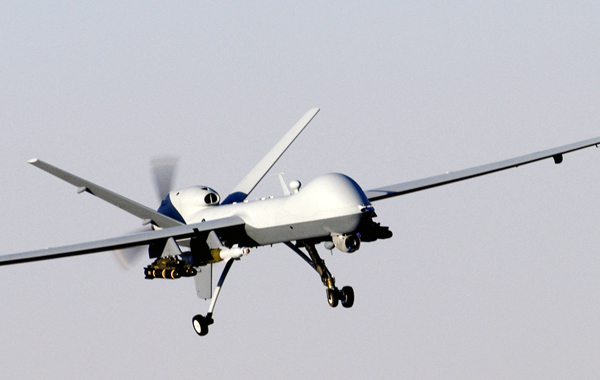
\includegraphics[width=7cm]{img/cap1/avion-espia}
  }
  \subfloat[Parrot AR-Drone]{
    \label{fig:drone}
    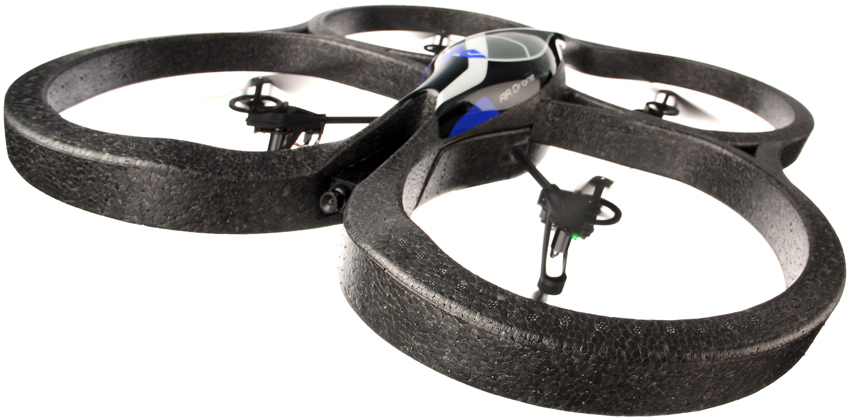
\includegraphics[width=7cm]{img/cap1/drone}
  }
  \caption{Distintos ejemplos de robots a�reos.}
\end{figure}

\item \textbf{Acu�ticos.} Estos robots se desplazan por encima o por debajo del agua. El m�todo de impulsi�n t�pico son las h�lices. Los submarinos rob�ticos se utilizan, por ejemplo, en tareas de reparaci�n o mantenimiento de cables interoce�nicos u oleoductos y exploraci�n del fondo marino. Los barcos rob�ticos se utilizan, sobretodo, en tareas militares de reconocimiento y vigilancia.

\begin{figure}[hbtp]
  \centering
  \subfloat[Barco rob�tico]{
    \label{fig:barcorobotico}
    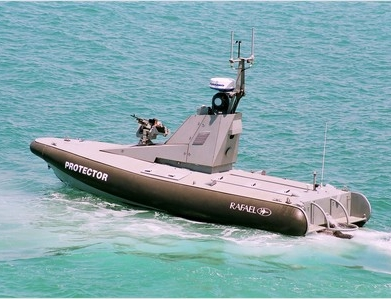
\includegraphics[width=7cm]{img/cap1/barcorobotico}
  }
  \subfloat[Submarino rob�tico]{
    \label{fig:submarinorobotico}
    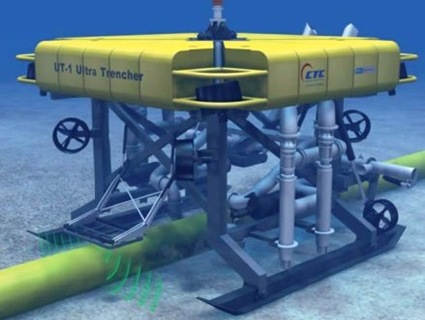
\includegraphics[width=7cm]{img/cap1/submarinorobotico}
  }
  \caption{Distintos ejemplos de robots acu�ticos.}
\end{figure}

\item \textbf{Espaciales.} Este tipo de robots se utilizan en el espacio. La mayor parte de ellos se utilizan en tareas de reconocimiento y de investigaci�n. La sonda Curiosity (Figura \ref{fig:curiosity}) es un robot h�brido, ya que, aparte de ser un robot espacial (su misi�n es reconocer y estudiar la superficie de Marte para determinar su habitabilidad), es un robot terrestre. El principal problema que presentan las sondas espaciales, sean del tipo que sean, es el retardo en la comunicaci�n entre �sta y la Tierra debido a la distancia. Es por esto que una caracter�stica muy importante en este tipo de robots es la autonom�a.
\end{itemize}

Todos los robots m�viles, independientemente del medio de locomoci�n que incorporen, comparten una serie de problemas comunes derivados del hecho de desplazarse y compartir su entorno con humanos. Entre estos problemas, destacamos:

\begin{itemize}

\item \textbf{Localizaci�n.} Consiste en averiguar d�nde nos encontramos dentro de entorno conocido. En exteriores ese problema est� resuelto gracias a la se�al GPS. El dispositivo GPS calcula la posici�n donde se encuentra gracias a una red de sat�lites que orbitan alrededor de la Tierra y que emiten cada uno una se�al. Esta se�al es recibida por el dispositivo y por ''triangulaci�n'' calcula la posici�n donde se encuentra, a�n as� la precisi�n es pobre, por lo que se utiliza junto a otros m�todos de localizaci�n para que sea m�s exacta. En interiores el problema de la localizaci�n se complica. Como la se�al GPS no suele recibirse correctamente dentro de edificios este m�todo no es adecuado. En este tipo de entornos suelen utilizarse algoritmos probabil�sticos que calculan su posici�n a partir de su informaci�n sensorial. Esta posici�n puede calcularse en un mapa construido \textit{a priori}, o que se construye en el proceso de localizaci�n como SLAM (Simultaneous Localization And Mapping). La informaci�n utilizada por estos algoritmos suele ser la proporcionada por los l�ser, los ultrasonidos, las c�maras o la odometr�a. Este entorno suele ser bastante cambiante, lo que provoca que el robot perciba objetos o personas que temporalmente se encuentren en medio y hagan que el robot no pueda calcular con precisi�n su posici�n.

\item \textbf{Navegaci�n.} Esta consiste en atravesar un entorno evitando los obst�culos para llegar a un destino. La navegaci�n se divide en dos: navegaci�n global y navegaci�n local. La navegaci�n global consiste en alcanzar una meta utilizando un mapa. Este puede conocerse \textit{a priori} o construirse autom�ticamente. Los algoritmos de navegaci�n global localizan al robot en este mapa y los destinos que debe alcanzar el robot suelen ser lejanos. Una de las t�cnicas m�s utilizada es la planificaci�n de caminos. La navegaci�n local se encarga de dirigir al robot sin utilizar un mapa. Esta navegaci�n esta basada en sensores y los destinos suelen ser cercanos. Los algoritmos de navegaci�n local deben de ser reactivos para poder reaccionar ante imprevistos. Los algoritmos m�s populares son CVM (m�todo de Velocidad y Curvatura), LVM (m�todo de Carriles y Velocidad), VFF (campos de potencial) y superposici�n de campos.

\item \textbf{Interacci�n hombre-m�quina.} Este problema es mucho m�s abierto y abstracto que los otros dos, de hecho, abarca multitud de campos como la psicolog�a, la inteligencia artificial, la rob�tica, la medicina o las humanidades, entre otros. El objetivo de la interacci�n hombre-m�quina consiste en realizar el intercambio de informaci�n entre el robot y el hombre de la forma m�s eficiente posible minimizando los errores y aumentando la productividad. Las interfaces para comunicarse con un robot deben ser lo m�s completas posibles, sin perder de vista la simplicidad y la intuitividad. El problema de la interacci�n hombre-m�quina es cr�tico, ya que puede hacer fracasar un proyecto con unos resultados muy buenos por requerir un proceso de aprendizaje del sistema demasiado complejo. La rob�tica social, de la cual hablaremos en la siguiente secci�n, es un ejemplo donde la capacidad de interactuar con el robot de una manera simple e intuitiva es vital.\\

\item \textbf{Coordinaci�n.} La coordinaci�n entre varios robots es un problema que a�n no se ha resuelto eficientemente. El objetivo es que un grupo de robots realicen una tarea interactuando unos con otros. Actualmente se est� investigando en controles de robots colaborativos basados en reglas.\\

\end{itemize}

\section{Rob�tica social}
\label{sec:roboticasocial}

Un robot social es un robot que interact�a con personas y se comunica con ellas siguiendo comportamientos, patrones y normas sociales. Una de las caracter�sticas f�sicas m�s importantes en este tipo de robots es la apariencia. �sta debe ser aceptada por un humano, por lo que se recurre a robots con aspecto humanoide o animal conocido. Tambi�n es muy importante que presenten rasgos agradables y atractivos, para no producir un rechazo en los usuarios.\\

\begin{figure} [hbtp]
  \begin{center}
    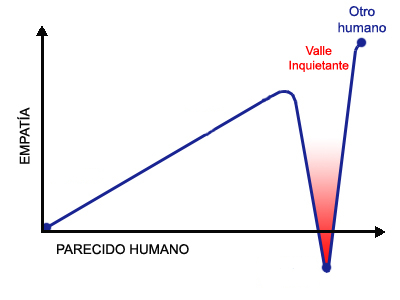
\includegraphics[width=9cm]{img/cap1/valleinquietante}
  \end{center}
  \caption{Teor�a del valle inquietante expuesta por el japon�s Masahiro Mori.}
  \label{fig:valleinquietante}
\end{figure}\

Un fen�meno interesante y de gran impacto en la relaci�n hombre-m�quina es el fen�meno de la teor�a del valle inquietante (Figura \ref{fig:valleinquietante}). Fue expuesta por el japon�s Masahiro Mori en 1970, \cite{Masahiro70}. Esta teor�a refleja la respuesta emocional de una persona hacia un robot con apariencia humana. Cuanto mayor es el parecido con un ser humano, la respuesta emocional y emp�tica crece hasta alcanzar un punto en el que se produce el efecto contrario, provocando rechazo. Una vez que el robot es indistinguible de un ser humano la respuesta emocional vuelve a crecer de forma positiva. Una posible explicaci�n a este fen�meno es que en un robot que no parezca una persona, las caracter�sticas humanas se ven m�s resaltadas, mientras que uno con apariencia casi igual a una persona se resaltan las contrarias, las caracter�sticas no humanas. Es decir, se ve al robot como una especia de ''zombie'' que produce rechazo. Es la misma reacci�n que se produce al observar un cad�ver. Por esto es muy importante la apariencia de los robots sociales. �sta debe ser agradable y amistosa, que no se vea como una amenaza para el usuario. La apariencia del robot puede marcar la diferencia entre el �xito o el fracaso de una investigaci�n o una aplicaci�n rob�tica, ya que si de primeras el robot no es aceptado, probablemente el proyecto fracase.\\

\begin{figure} [hbtp]
  \begin{center}
    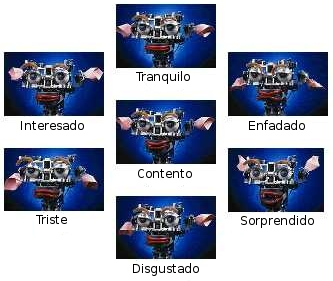
\includegraphics[width=12cm]{img/cap1/kismet}
  \end{center}
  \caption{Expresiones faciales del robot Kismet.}
  \label{fig:kismet}
\end{figure}\

El primer robot cuyo principal objetivo era interactuar con humanos es Kismet, \cite{Breazeal99} y \cite{Breazeal2000}. Kismet es un robot capaz de realizar la interacci�n social b�sica que tienen las personas leyendo las emociones a trav�s de la voz. En cualquier idioma, un comentario positivo tiene un tono distinto al de un comentario negativo. Kismet puede comprender el tono de voz e interpretarlo. Este robot tambi�n sabe expresar sus emociones por medio de gestos de la cara. Por ejemplo, cuando est� cansado inclina los ojos hacia abajo, en cambio si est� contento se sienta erguido y sonr�e. Se produce una interacci�n entre el robot y el humano natural obteniendo una comunicaci�n m�s emp�tica. En la figura \ref{fig:kismet} pueden verse distintas expresiones del robot.\\

Otro robot social es Paro. Se trata de una foca rob�tica utilizada para prop�sitos terap�uticos con pacientes discapacitados, ancianos o ni�os autistas en centros hospitalarios o residencias de mayores, \cite{Shibata2003} y \cite{Shibata2009}. Este robot dispone de varios sensores que le permiten interactuar con la persona que lo utiliza. Dispone de un sensor de luz con el que reconoce la oscuridad o la luz. Gracias a los sensores t�ctiles es capaz de reconocer si es acariciado o tocado y responder a esos est�mulos. Tambi�n reconoce la direcci�n de la voz y algunas palabras como su nombre, saludos o mimos. Este robot se ha utilizado en terapias reales con pacientes de autismo con resultados positivos. En la figura \ref{fig:paro} se puede ver al robot Paro en una sesi�n terap�utica.\\

En la misma l�nea de rob�tica social que siguen estos robots se plantea el presente proyecto: la utilizaci�n del robot Nao como herramienta terap�utica en sesiones de terapia ocupacional para pacientes con la enfermedad de Alzheimer. En este contexto surge el t�rmino roboterapia, que consiste en la utilizaci�n de robots en terapias ocupacionales con pacientes.\\

\begin{figure} [hbtp]
  \begin{center}
    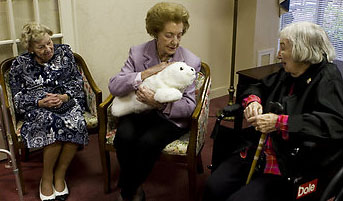
\includegraphics[width=12cm]{img/cap1/paro}
  \end{center}
  \caption{Sesi�n terap�utica con ancianos y el robot Paro.}
  \label{fig:paro}
\end{figure}\

\section{Estructura de este documento}
\label{sec:estructura}

En esta memoria se detallan todos los aspectos relevantes del desarrollo de esta investigaci�n. La memoria est� dividida en seis cap�tulos. En este primer cap�tulo se ha presentado el entorno en el que se realiza el estudio, se ha introducido la rob�tica en general y se ha definido qu� es la rob�tica social. En el segundo cap�tulo se expone el problema al que nos enfrentamos y se comentan los objetivos y requisitos planteados para el proyecto. En el tercer cap�tulo se detalla la infraestructura software sobre la que se ha construido este proyecto y el hardware utilizado. La implementaci�n y los detalles t�cnicos relativos al proyecto se encuentran en el cuarto cap�tulo. Con el fin de mostrar los efectos y la viabilidad de esta investigaci�n en el quinto cap�tulo se ofrecen una serie de experimentos. Por �ltimo, en el sexto cap�tulo se presentan las conclusiones extra�das y se proponen nuevas l�neas de investigaci�n futuras.

















% Capitulo 2
\chapter{Objetivos y Metodolog�a}
\label{cap:objetivos}

Una vez presentado el contexto en el que se sit�a la investigaci�n, en este cap�tulo se fijan los objetivos y requisitos del proyecto. Para ello primero se describir� el problema al que nos enfrentamos, que es la introducci�n de un robot en terapias ocupacionales para enfermos de Alzheimer, y luego se fijar�n los objetivos y requisitos en base al problema. Por �ltimo, explicaremos la metodolog�a seguida, el plan de trabajo que se ha llevado a cabo y el calendario de sesiones que se ha seguido.

\section{Descripci�n del problema}
\label{sec:descripcionproblema}

La enfermedad de Alzheimer es un tipo de demencia senil que, como todas ellas, afecta a las funciones del cerebro. Se caracteriza por una p�rdida progresiva de la memoria, de la capacidad de razonar y de la conducta. La enfermedad de Alzheimer es la forma m�s com�n de demencia y afecta, sobretodo, a las personas mayores de 65 a�os. Aproximadamente un 12\% de la poblaci�n mayor de 65 a�os tiene esta enfermedad. El n�mero de enfermos de Alzheimer ha crecido mucho en los �ltimos a�os debido, principalmente, por el aumento de la esperanza de vida, que actualmente en Espa�a est� en 81,5 a�os.\\

Las causas de esta enfermedad siguen siendo desconocidas, pero lo que s� se conocen son los factores de riesgo. Como acabamos de comentar la edad es un factor importante junto a la gen�tica y los antecedentes familiares. Las personas con s�ndrome de Down tambi�n tienen un riesgo muy alto de padecer esta enfermedad. La enfermedad de Alzheimer parece ser m�s com�n en mujeres que en hombres, de hecho, casi dos tercios de las personas que sufren esta enfermedad son mujeres.\\

Desgraciadamente en la actualidad, no existe cura para esta enfermedad. En su lugar los tratamientos se enfocan en aliviar y retrasar la progresi�n de los s�ntomas, como la p�rdida de memoria. Adem�s del tratamiento farmacol�gico correspondiente, se ha comprobado que la participaci�n en terapias ocupacionales por parte de los pacientes es algo muy beneficioso. Estas terapias est�n orientadas al desarrollo de diferentes actividades en las que se les incita a realizar ciertas actividades cognitivas y f�sicas.\\

Hace tres a�os le surgi� la oportunidad al grupo de rob�tica de la Universidad Rey Juan Carlos de participar en estas terapias incluyendo al robot como herramienta terap�utica. A estas terapias se les ha dado el nombre de Roboterapia. El objetivo de este proyecto, como veremos a continuaci�n, gira en torno a este tema.\\

Al introducir un robot en terapias ocupacionales de enfermos de Alzheimer surgen una serie de problemas que intentaremos resolver en el desarrollo del proyecto. La interacci�n con un robot no siempre es f�cil ni intuitiva, por lo que el conjunto de herramientas debe ser f�cil de usar. Las sesiones se realizan en base a unos guiones que se elaboran previamente, as� que las herramientas deben elaborarse en torno a la ejecuci�n de �stos porque son el pilar fundamental de una sesi�n. A continuaci�n, se presentan los objetivos que se han propuesto para este proyecto. 

\section{Objetivo del proyecto}
\label{sec:objetivoproyecto}

El objetivo principal del proyecto es el de desarrollar un conjunto de herramientas que ayude a los terapeutas a usar un robot durante la realizaci�n de terapias ocupacionales con enfermos de Alzheimer, es decir, realizar sesiones de roboterapia. Las herramientas deben ser lo suficientemente simples e intuitivas como para permitir a los terapeutas usar el robot sin dejar de prestar atenci�n a los enfermos. Adem�s de estas herramientas, el sistema puede emplear cualquier m�todo de control externo que facilite dicha tarea.\\

Este objetivo principal se ha dividido en varios subobjetivos para simplificar el desarrollo del proyecto y asegurarnos que se llevan a cabo correctamente:

\begin{enumerate}
\item \textbf{Terapias.} La herramientas ser�n capaces de reproducir varias terapias desarrolladas por los investigadores encargados de la investigaci�n en la Fundaci�n CIEN. Las acciones interesantes para el reproductor de terapias son cargar terapias, ejecutar la acci�n siguiente y reproducir la acci�n que se quiera.

\item \textbf{Herramientas de teleoperaci�n.} Se debe poder teleoperar al robot para, en caso necesario, controlarlo y que ejecute las acciones que el terapeuta crea convenientes. Las acciones que nos interesan son desplazar al robot, controlar la cabeza, reproducir sonidos y efectuar movimientos.

\item \textbf{Herramientas de control auxiliares.} Se incorporar� un m�todo de control externo para facilitar el manejo del robot a los terapeutas encargados de hacer la terapia y permitir que sean aut�nomos. El dispositivo debe ser inal�mbrico y f�cil de usar.

\item \textbf{Integraci�n.} Todo ello debe ir integrado en una sola aplicaci�n con un interfaz gr�fico simple. Se tendr� en cuenta que la aplicaci�n ser� usada por profesionales de la medicina, no inform�ticos.
\end{enumerate}

Durante todo el proceso de desarrollo habr� una realimentaci�n continua por parte de los terapeutas y los m�dicos de la Fundaci�n. El software ser� probado todas las semanas en las sesiones de Roboterapia programadas por la Fundaci�n CIEN.\\

\section{Requisitos}
\label{sec:requisitos}

El desarrollo de este proyecto, siguiendo la l�nea marcada por los objetivos, deber� ajustarse y cumplir los siguientes requisitos:

\begin{enumerate}
\item El lenguaje de programaci�n para la interfaz gr�fica ser� Java.
\item Las herramientas correr�n sobre un sistema GNU/Linux. La elecci�n de la distribuci�n es libre.
\item La interfaz gr�fica deber� ser simple e intuitiva. Se debe tener en cuenta que los usuarios de las herramientas probablemente no dispongan de conocimientos inform�ticos avanzados.
\item El robot se ejecutar� bajo una versi�n de BICA, que es una arquitectura software de componentes iterativos basada en comportamiento, creada en el grupo de Rob�tica de la Universidad y que permite programar el robot Nao eficazmente. Este software se describe m�s adelante, en la secci�n \ref{sec:bica}.
\item Se incorporar� un dispositivo externo que facilite el manejo del robot y aporte autonom�a al terapeuta.
\end{enumerate}

\section{Metodolog�a y planificaci�n}
\label{sec:metodologiaplanificacion}

La metodolog�a escogida para la realizaci�n de este proyecto es el \textit{modelo de prototipos}. Se trata de un modelo de desarrollo evolutivo. Este tipo de modelos se caracteriza por ser un modelo iterativo en el que los requisitos del cliente no son completamente conocidos al inicio del proyecto. El modelo de prototipos, como su nombre indica, se basa en la construcci�n de prototipos. Un prototipo se puede definir como una versi�n preliminar de un sistema con fines demostrativos o de evaluaci�n. La idea principal de este modelo es desarrollar una implementaci�n inicial (prototipo), someterla a la evaluaci�n del usuario y refinarla por medio de diferentes versiones. Los prototipos deben ser construidos en poco tiempo y no deben consumir demasiados recursos.\\

Como se puede ver en la figura \ref{fig:modeloprototipos}, se parte de una breve descripci�n de lo que quiere el cliente. Las actividades de especificaci�n, desarrollo y validaci�n se realizan conjuntamente con una retroalimentaci�n r�pida entre ellas. De cada una de las revisiones se obtiene un prototipo que es evaluado por el cliente o el usuario y comienza de nuevo el proceso.\\

\begin{figure} [hbtp]
  \begin{center}
    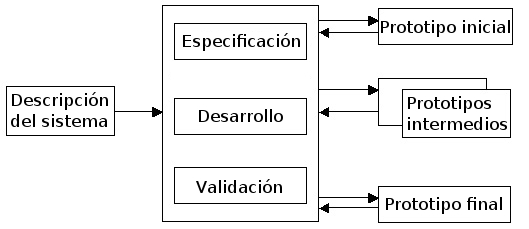
\includegraphics[width=12cm]{img/cap2/modeloprototipos}
  \end{center}
  \caption{Modelo de desarrollo de prototipos.}
  \label{fig:modeloprototipos}
\end{figure}

El enfoque de prototipos suele ser m�s efectivo que otros m�s est�ticos, como el modelo en cascada, porque satisface las necesidades inmediatas del cliente. Para sistemas peque�os y de tama�o medio, se ha comprobado que los enfoques evolutivos de desarrollo son los que mejores resultados devuelven. Pero no todo son ventajas, el modelo de prototipos tiene algunos inconvenientes. Al crear los prototipos de forma r�pida, se suelen desatender aspectos importantes del software como la calidad, el mantenimiento a largo plazo y la documentaci�n: Adem�s,los continuos cambios en los requisitos para cada prototipo contribuyen a que el sistema tenga una estructura deficiente.\\

Pese a los inconvenientes que acabamos de mencionar, creemos que este modelo de desarrollo es el que m�s se ajusta a nuestras necesidades. El proyecto que se presenta en esta memoria es un proyecto de investigaci�n donde los requisitos suelen cambiar bastante. Este modelo nos permite ajustarnos a estos cambios y desarrollar con rapidez un nuevo prototipo. Es conveniente recordar que la realizaci�n de las terapias se efectuar� al mismo tiempo que el desarrollo del proyecto. Adem�s, se mantendr�n reuniones semanales con el tutor del proyecto para comentar los resultados obtenidos y planificar el siguiente prototipo.

\subsection{Plan de trabajo}
\label{subsec:plantrabajo}

En este apartado se explica el plan de trabajo seguido. Se ha dividido en distintas fases para simplificar el trabajo. Como resultado final de cada fase se obtiene un resultado, ya sea un prototipo o conocimiento adquirido.\\

Seg�n se define en la norma escrita por el IEEE sobre procesos del ciclo de vida del software, \cite{iso12207}: \textit{Un prototipo es una versi�n limitada del producto que permite a las partes responsables de su creaci�n probarlo en situaciones reales y explorar su uso}. Como hemos comentado previamente en el cap�tulo, hemos seguido la metodolog�a de desarrollo de prototipos. Como resultado de cada fase se obtiene un prototipo que es probado y evaluado para poder mejorarlo en la siguiente iteraci�n. Para simplificar m�s algunas iteraciones complejas como la primera, hemos dividido este esfuerzo en varias iteraciones, por lo que el resultado de estas no siempre es un prototipo, tambi�n puede ser adquisici�n de conocimiento.

\begin{itemize}
\item \textbf{Fase 1.} Familiarizaci�n con el entorno y primer prototipo. Esta primera fase requiere bastante esfuerzo por lo que est� dividida a su vez en varias iteraciones. �sta consiste, \textit{grosso modo}, en crear el primer prototipo pero para ello hay que familiarizarse con el entorno.
  \begin{itemize}
  \item \textbf{Fase 1.1.} Familiarizaci�n con el Software. En esta primera subiteraci�n se realizar� un primer acercamiento a BICA, que es el software creado en el grupo de Rob�tica para el robot. Los tres elementos software que estudiaremos son \textit{Player}, \textit{Jmanager} y el motor de comunicaciones \textit{ICE}.
  \item \textbf{Fase 1.2.} Familiarizaci�n con el Hardware. En esta segunda subiteraci�n nos centraremos en el robot, tanto en su configuraci�n como en la comunicaci�n con �l a trav�s de \textit{ICE}.
  \item \textbf{Fase 1.3.} Asistencia a una sesi�n de roboterapia acompa�ado. Se asistir� a una primera sesi�n de terapia acompa�ado por el tutor del proyecto. El objetivo de esta subiteraci�n es conocer el entorno en el que se desarrollan las terapias para comprender mejor el problema.
  \item \textbf{Fase 1.4.} Elaboraci�n del primer prototipo. Una vez adquirido el conocimiento m�nimo de los aspectos b�sicos del problema, se puede crear el primer prototipo. Una vez elaborado, el software se  probar� en una sesi�n real de roboterapia y se evaluar�n los resultados para una posterior mejora.
  \end{itemize}
\item \textbf{Fase 2.} Esta fase, aunque se haya representado como una sola, est� compuesta por varias. Consiste en, a partir de los resultados obtenidos en la evaluaci�n del prototipo anterior, redise�ar el componente software para adaptarlo a los cambios sugeridos y a�adir las nuevas funcionalidades. Este nuevo prototipo ser� probado en una nueva sesi�n de roboterapia y posteriormente ser� evaluado. Esta fase se repetir� durante todo el proyecto. 
\item \textbf{Fase 3.} La �ltima fase se ha separado por ser un poco diferente de las iteraciones de la fase 2. Una vez finalizadas las terapias se crear� una peque�a documentaci�n del �ltimo prototipo para poder cerrar la investigaci�n. Este �ltimo punto es importante para retomar la investigaci�n en un futuro.
\end{itemize}

\begin{table}[htbp]
\begin{tabular}{|l||c|c|c|c|c|c|c|} 
\hline
Mes/D�a & Lunes & Martes & Mi�rcoles & Jueves & Viernes & S�bado & Domingo \\ \hline \hline
Junio & & & \cellcolor[gray]{0.8} 1.1 & & & & \\ \hline
Julio & & & \cellcolor[gray]{0.8} 1.1 & & & & \\ \hline
Agosto & & & \cellcolor[gray]{0.8} 2.2 & \cellcolor[gray]{0.8} 1.5 & & & \\ \hline
Septiembre & & \cellcolor[gray]{0.8} CD & \cellcolor[gray]{0.8} 2.2 & \cellcolor[gray]{0.8} 1.5 & & & \\ \hline
Octubre & & \cellcolor[gray]{0.8} CD & \cellcolor[gray]{0.8} 2.2 & & & & \\ \hline
Noviembre & & \cellcolor[gray]{0.8} CD & & & & & \\ \hline
\end{tabular}
\caption{Calendario de las sesiones que se realizar�n para la investigaci�n.}
\label{tab:calendario}
\end{table}

Las terapias se realizar�n entre los meses de junio y noviembre, ambos inclusive. La frecuencia de las terapias y la unidad en la que se har� est� marcada por los investigadores de la Fundaci�n CIEN, reflejado en el calendario de la tabla \ref{tab:calendario}. En la residencia, los pacientes de Alzheimer est�n agrupados en unidades seg�n el grado de desarrollo de la enfermedad. En la unidad 1.1 se encuentran los enfermos leves, en la 1.5 los enfermos moderados y en la 2.2 los m�s graves. CD corresponde a ''Centro de d�a''. El Centro de d�a est� compuesto por ancianos que no duermen en la residencia. La mayor�a de ellos se encuentra en estad�os iniciales de la enfermedad de Alzheimer.\\

Cada d�a de terapia se har�n dos sesiones en el mismo grupo, una de terapia ocupacional y otra de fisioterapia. Todas las sesiones ser�n grabadas con c�mara de v�deo para su posterior evaluaci�n. Estas grabaciones no influyen en nuestro proyecto, solamente se usar�n para evaluaciones m�dicas de las terapias.\\







% Capitulo 3
\chapter{Entorno y plataforma de desarrollo}
\label{cap:entorno}

En este cap�tulo se describen los elementos hardware y software utilizados en el proyecto. En la figura \ref{fig:bloques-app} se puede ver un esquema con las conexiones entre los distintos elementos que componen el sistema.\\

\begin{figure} [hbtp]
  \begin{center}
    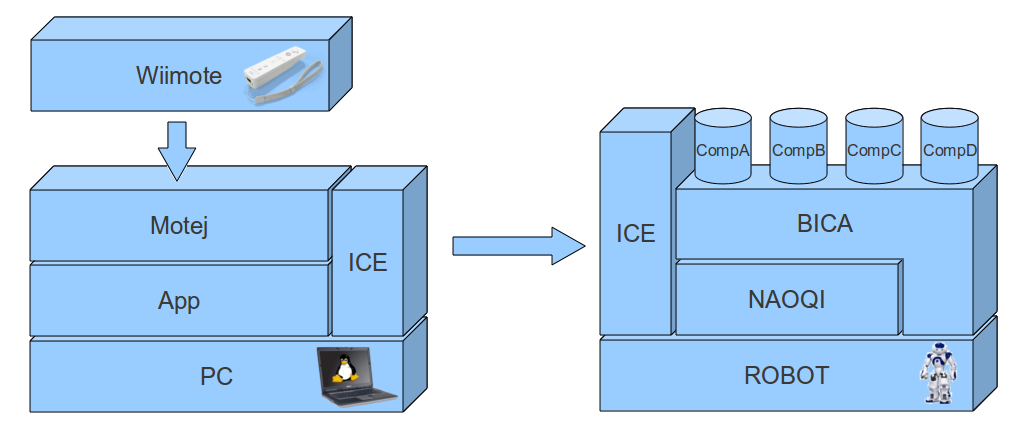
\includegraphics[width=15cm]{img/cap3/bloques-app}
  \end{center}
  \caption{Esquema de la aplicaci�n.}
  \label{fig:bloques-app}
\end{figure}\

En el lado derecho de la figura tenemos los componentes software que se ejecutan en el robot. La capa inferior representa al robot con sus actuadores y sensores. Sobre �sta se encuentra \textit{NaoQi}\footnote{http://www.aldebaran-robotics.com/en/Discover-NAO/Key-Features/NAOqi.html}, que es un Framework que facilita el acceso a los sensores y actuadores del robot. Por encima de \textit{NaoQi} est� BICA. BICA es una arquitectura software, desarrollada por el grupo de Rob�tica de la Universidad, que permite definir el comportamiento del robot mediante la ejecuci�n de componentes software. Los componentes son las piezas software que contienen la funcionalidad real del robot. Para poder modular su ejecuci�n desde una plataforma exterior se utilizan las interfaces proporcionadas por ICE, que es un motor de comunicaciones de Internet.\\

En el lado izquierdo de la figura se encuentran los componentes software que permiten manejar al robot. La aplicaci�n que se ha desarrollado en este proyecto se ejecuta sobre un PC con un sistema GNU/Linux instalado en �l. Para modular y monitorizar los distintos componentes de BICA se utilizan las interfaces ICE proporcionadas por BICA. La conexi�n con el Wiimote se realiza a trav�s de la biblioteca \textit{Motej}\footnote{http://motej.sourceforge.net}, biblioteca de software libre disponible en la red. La conexi�n entre el robot y la aplicaci�n es WiFi, mientras que la conexi�n entre el Wiimote y la aplicaci�n es bluetooth.\\

A continuaci�n se exponen en profundidad estos elementos y, en particular, aquellos relevantes en este proyecto.

\section{Robot Nao}
\label{sec:robotnao}

Nao es un robot humanoide de 58 cm de altura (Figura \ref{fig:gradoslibertad}). Lo desarrolla la empresa francesa \textit{Aldebaran Robotics}\footnote{http://www.aldebaran-robotics.com/}. El proyecto de desarrollo del Nao nace en 2004. Al poco tiempo, en 2007, reemplaza al robot Aibo, creado por Sony, como el robot usado en la competici�n de la \textit{RoboCup Standard Platform League (SPL)}. En 2011 Aldebaran anuncia que van a lanzar el c�digo fuente del controlador del Nao como software libre. Por el momento este robot es utilizado mayoritariamente en el �mbito acad�mico, pero fuera de �ste tiene muchos usos a�n por descubrir. Las principales caracter�sticas del robot Nao son:

\begin{packed_item}
\item Gran cantidad de movimientos. El \textit{Nao Robocup Edition}, que es la versi�n utilizada para la Robocup y la que se utiliza en este proyecto, cuenta con 21 grados de libertad.
\item Detectores de presi�n en pies y manos, conocidos como FSR, \textit{Force Sensitive Resistors}. Este dispositivo tiene la capacidad de disminuir su resistencia cuando aumenta la fuerza aplicada sobre �l. Suele utilizarse para el control de dispositivos electr�nicos con el tacto.
\item Dos c�maras situadas en la cabeza con distintas zonas de visi�n. Una de ellas est� situada en la frente del robot y apunta hacia el frente. La otra c�mara esta situada en la boca del robot y tiene cierta inclinaci�n hacia abajo. Los �ngulos de visi�n de las c�maras no se solapan, en la figura \ref{fig:zonasvision} se puede ver hacia donde apunta cada c�mara. Ambas tienen una resoluci�n HD, 640x480 p�xeles.
\item Cuatro sensores de ultrasonido colocados en el pecho del robot.
\item Un sensor inercial que mide la aceleraci�n y la velocidad angular. Este sensor es muy �til en caso de ca�das para detectarlas y actuar en consecuencia.
\item Interfaces de red Ethernet y WiFi que aportan conectividad al robot.
\item LEDs con distintos colores repartidos por el cuerpo del robot. Tiene uno en el bot�n de encendido y apagado del pecho del robot, un par en los ojos y varios en las orejas y pies.
\item Cuatro micr�fonos colocados en la parte frontal, la parte posterior, al lado derecho y al lado izquierdo del robot.
\item Dos altavoces Hi-Fi en est�reo para reproducir sonidos colocados en la cabeza del robot.
\end{packed_item}

\begin{figure}[hbtp]
  \centering
  \subfloat[Sensores y actuadores del robot.]{
    \label{fig:gradoslibertad}
    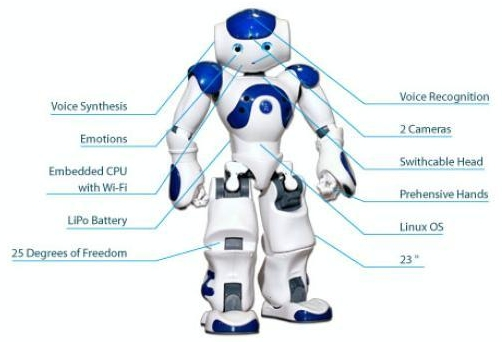
\includegraphics[width=9cm]{img/cap3/gradoslibertad}
  }
  \subfloat[Zonas de visi�n de cada una de las c�maras.]{
    \label{fig:zonasvision}
    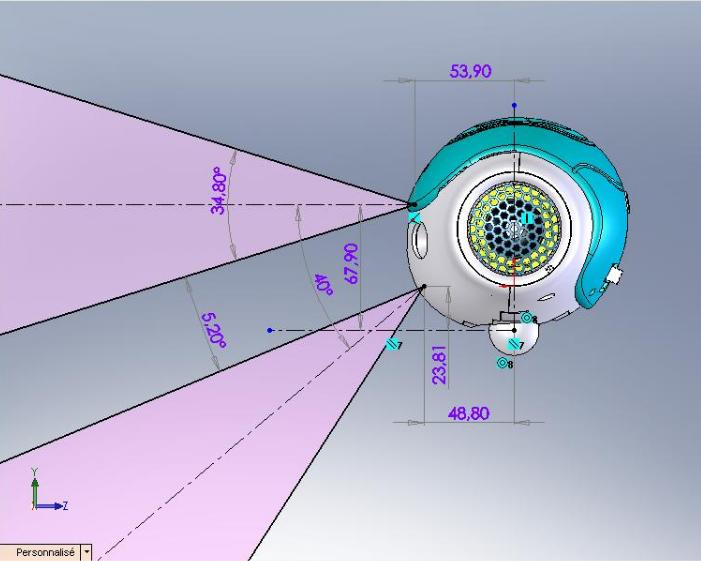
\includegraphics[width=6cm]{img/cap3/zonasvision}
  }
  \caption{El robot Nao.}
  \label{fig:robotnao}
\end{figure}

El robot dispone de un procesador x86 AMD Geode 500MHz y usa como sistema operativo Linux. Se alimenta de una bater�a recargable que le permite funcionar durante aproximadamente 45 minutos o durante quince minutos caminando sin parar. Este tiempo es suficiente ya que las sesiones de Roboterapia duran entre 30 y 40 minutos.\\

La caracter�stica m�s importante del robot y por la que fue elegido es por su aspecto f�sico. El robot tuvo que pasar una serie de pruebas de aceptaci�n por parte de los pacientes antes de poder empezar a realizar las terapias con �ste. Gracias al peque�o tama�o y el aspecto amigable que tiene, el robot no representa una amenaza ni produce rechazo, por lo que pas� las pruebas con �xito y se pudieron comenzar las terapias.

\section{NaoQi}
\label{sec:naoqi}

\textit{NaoQi} es un Framework, creado por Aldebaran Robotics, que permite desarrollar aplicaciones en C++ y Python en el Nao. Facilita el acceso a los sensores y actuadores del robot. Las aplicaciones creadas pueden ser ejecutadas directamente por el robot o remotamente en un ordenador.\\

Los ejecutables creados con este Framework se llaman \textit{broker}. Los \textit{broker} se ejecutan de forma independiente y se encuentran escuchando en una direcci�n IP y un puerto, por lo que pueden ser ejecutados en el propio robot, usando un compilador cruzado proporcionado por el Framework, o remotamente desde un ordenador. Un \textit{broker} esta formado por una serie de m�dulos que ofrecen distintas funcionalidades. Las funciones de estos m�dulos pueden ser llamadas desde otros m�dulos o incluso desde otros \textit{broker}.\\

\begin{figure} [hbtp]
  \begin{center}
    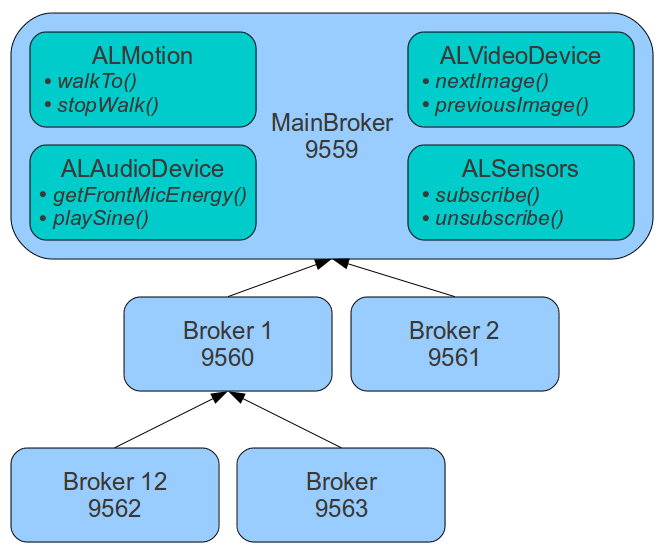
\includegraphics[width=9cm]{img/cap3/broker-naoqi}
  \end{center}
  \caption{Arquitectura de NaoQi modulada por medio de \textit{Brokers}.}
  \label{fig:broker-naoqi}
\end{figure}\

En la figura \ref{fig:broker-naoqi} se puede ver un esquema de la arquitectura de \textit{NaoQi} modulada por medio de los \textit{broker}. El \textit{broker} m�s importante es el \textit{MainBroker} porque nos da acceso a los sensores y actuadores del robot. Cuando se desarrolla una aplicaci�n para el robot con este Framework, se puede ejecutar a trav�s de un \textit{broker} propio o como un m�dulo del \textit{MainBroker}; BICA se ejecuta de esta �ltima manera. \textit{NaoQi} se utiliza para acceder a los sensores y actuadores de una manera m�s sencilla.\\

Los \textit{brokers} se organizan internamente en m�dulos. Cada uno de estos m�dulos aporta una funcionalidad concreta o permite acceder a sensores o actuadores del robot. Por ejemplo, \texttt{ALMotion} proporciona m�todos que facilitan hacer que el robot se mueva; \texttt{ALAudioDevice} contiene otros m�dulos de \textit{NaoQi} que nos dan acceso a las entradas y salidas de audio; \texttt{ALVideoDevice} se encarga de proporcionar im�genes de las c�maras, y \texttt{ALSensors} es responsable de lanzar los eventos correspondientes cuando se pulsa un bot�n o se tocan las zonas t�ctiles de la cabeza o las manos.

\section{BICA}
\label{sec:bica}

BICA\footnote{http://www.robotica-urjc.es/index.php/Robocup}, \textit{Behavior-based Iterative Component Architecture}, es un software desarrollado en el grupo de Rob�tica de la Universidad Rey Juan Carlos, \cite{BICA2010}. Se trata de una plataforma de desarrollo de software para el robot Nao. En el bloque situado a la derecha de la figura \ref{fig:bloques-bica} se puede ver la arquitectura de BICA dividida en capas.

\begin{figure} [hbtp]
  \begin{center}
    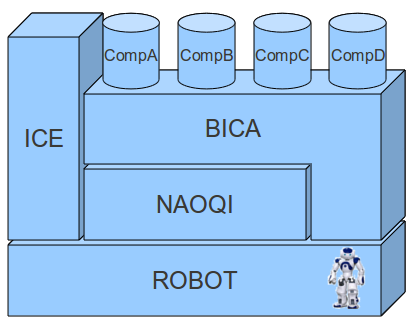
\includegraphics[width=7cm]{img/cap3/bloques-bica}
  \end{center}
  \caption{Arquitectura de BICA dividido en capas.}
  \label{fig:bloques-bica}
\end{figure}\

La unidad b�sica en la arquitectura de BICA es el \textit{componente}, representado en la figura \ref{fig:componente-bica}. La funcionalidad de los \textit{componentes} puede ser implementada mediante una m�quina de estados o pueden ser controladores reactivos, es decir, que ejecutan al momento la acci�n requerida. Los \textit{componentes} pueden activarse o desactivarse. Un \textit{componente} activo ejecuta una tarea determinada de manera iterativa y con una frecuencia previamente fijada. Los \textit{componentes} que est�n activos iteran y consumen recursos. Los \textit{componentes} tienen una serie de m�todos para modularlos y devuelven los resultados obtenidos.\\

\begin{figure} [hbtp]
  \begin{center}
    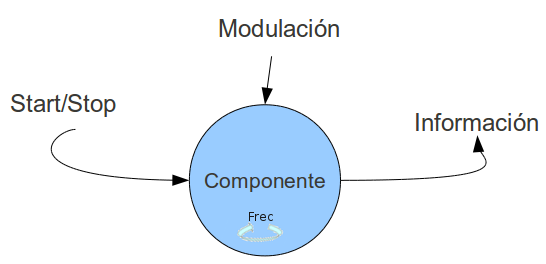
\includegraphics[width=9cm]{img/cap3/componente-bica}
  \end{center}
  \caption{Esquema de las entradas y salidas de un componente de BICA.}
  \label{fig:componente-bica}
\end{figure}

Para realizar tareas m�s complejas los \textit{componentes} pueden comunicarse entre s�. La arquitectura de BICA tiene una estructura jer�rquica, tal y como se muestra en la figura \ref{fig:componentes-bica}. Cuando se activa el \textit{Componente A}, �ste activa los \textit{componentes D} y \textit{E}. A su vez, el componente \textit{D} activa los \textit{componentes G} y \textit{H}, y el \textit{componente E} activa los \textit{componentes H}, \textit{I} y \textit{J}. Un \textit{componente} puede ser activado por varios \textit{componentes}. Aunque sea llamado repetidas veces, �ste se ejecutar� a la frecuencia m�nima que tenga configurada para evitar ciclos innecesarios y se ahorren recursos. Los \textit{componentes} de ''bajo nivel'', como los \textit{componentes G}, \textit{H}, \textit{I} y \textit{J}, se comunican directamente con el robot u obtienen la informaci�n mediante llamadas de \textit{NaoQi}.\\

\begin{figure} [hbtp]
  \begin{center}
    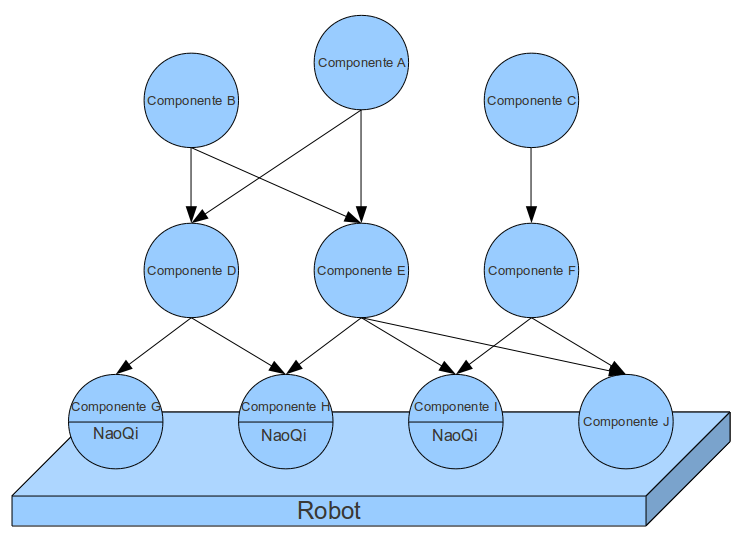
\includegraphics[width=9cm]{img/cap3/componentes-bica}
  \end{center}
  \caption{Jerarqu�a de componentes de BICA.}
  \label{fig:componentes-bica}
\end{figure}

A continuaci�n se muestra un ejemplo en pseudoc�digo muy b�sico del funcionamiento de los \textit{componentes}. Los \textit{componentes} tienen un par de m�todos indispensables: \texttt{init()} y \texttt{step()}. Desde el m�todo \texttt{init()} se inicializan los recursos necesarios ejecutar el \textit{componente}. El m�todo \texttt{step()} es el que activa el \textit{componente} y contiene toda su funcionalidad. Como el \textit{componente} se activa solamente cuando se llama a este m�todo, no es necesario ning�n otro m�todo para detener su ejecuci�n. Todos los \textit{componentes} disponen de un m�todo privado llamado \texttt{isTime2Run()} que nos modula la frecuencia a la que se ejecuta el \textit{componente}. Si a�n no tiene que ejecutarse el \textit{componente}, el m�todo devuelve \texttt{false} y no se ejecuta ninguna instrucci�n del \textit{componente}.

\begin{lstlisting}[style=C]
void step() {
  // Ejecuci�n en cascada de los componentes de los que se
  // obtienen informaci�n.
  cp1->step();
  cp2->step();

  if (isTime2Run()) {
    // Recoger datos de los componentes perceptivos.

    // Iteraci�n genuina

    // Poner a disposici�n del resto de componentes los datos
    // calculados y/o se modulan los componentes actuadores.
  }

  // Ejecuci�n en cascada de los componentes que se han
  // modulado o requieran ser ejecutados por su actuaci�n.
  ca1->step();
  ca2->step();
}
\end{lstlisting}

Al inicio del m�todo \texttt{step()} se llama a los \textit{componentes} perceptivos, son aquellos que devuelven datos, de los que depende el \textit{componente}. Si es el momento de que se ejecute el \textit{componente}, el m�todo \texttt{isTime2Run()} devuelve \textit{true} y se ejecutan las instrucciones dentro de la estructura \textit{if}. B�sicamente, lo que se hace en esta estructura es procesar los datos devueltos por los \textit{componentes} perceptivos y generar nuevos datos. En caso de que el \textit{componente} genere una respuesta, se modulan los \textit{componentes} actuadores, aquellos que generan una respuesta en el robot o procesan los datos que acabamos de crear. Por �ltimo, se llama al \texttt{step()} de �stos para que efect�en las acciones requeridas que acabamos de modular.\\

BICA est� desarrollado en C++ y consiste en una arquitectura iterativa, formada por \textit{componentes} y basada en comportamientos. Proporciona un entorno de programaci�n monohilo. Gracias a que se ejecuta en un s�lo hilo nos evita las condiciones de carrera, un error muy frecuente y dif�cil de detectar en la programaci�n concurrente.\\

Se ha escogido esta plataforma software por ser robusta y estar bastante probada. Ya ha sido utilizada en varios proyectos y es la plataforma utilizada en la RoboCup por el equipo de la universidad. Adem�s, dispone de varios \textit{componentes} que se pueden reutilizar para nuestro proyecto, de los cuales hablaremos en la secci�n \ref{sec:componentes}.\\

Las comunicaciones con agentes externos se realizan a trav�s del motor de comunicaciones de Internet, ICE, \textit{Internet Communications Engine}. Se trata de un \textit{middleware} de computaci�n distribuida, orientado a objetos, multiplataforma y es desarrollado por la empresa \textit{ZeroC}\footnote{http://www.zeroc.com/}. Este \textit{middleware} proporciona una soluci�n simple en el �mbito de las comunicaciones entre aplicaciones distribuidas en distintos servidores.\\

ICE dispone de una versi�n para sistemas embebidos, \textit{Ice-E}. Esta versi�n es un motor de comunicaciones m�s compacto dise�ado para ejecutarse en entornos de recursos limitados como tel�fonos inteligentes o PDAs, por poner un par de ejemplos. Esta es la versi�n utilizada en el robot, ya que los recursos son bastante limitados y se necesita que el software corra los m�s r�pidamente posible. Gracias a ICE, BICA puede comunicarse con \textit{JManager} o con otros robots que usen BICA.\\

\section{Componentes BICA}
\label{sec:componentes}

En esta secci�n se habla de los distintos \textit{componentes} de BICA que hemos utilizado en nuestra aplicaci�n, estos son: \textbf{Music}, \textbf{Body}, \textbf{Head} y \textbf{Movie}. La mayor�a de ellos est�n formados por una m�quina de estados. Los diagramas de m�quina de estados que se muestran en algunos componentes est�n sacados de la herramienta visual de dise�o de componentes BICA: VICODE, del cual se habla en la secci�n \ref{sec:jmanager}.\\ 

Los \textit{componentes} pueden definirse como m�quinas de estado. Los diagramas de la m�quina de estados de los \textit{componentes} se interpretan de la siguiente manera. El estado inicial est� representado con un c�rculo rojo. Todos los \textit{componentes} se inician en este estado cuando se activan. El resto de estados se representan mediante c�rculos amarillos. Las transiciones entre un estado y otro se representan con un c�rculo de menor tama�o y azul. Las flechas que entran y salen de este peque�o c�rculo indican el sentido de la transici�n entre dos estados. Cuando en el estado de un \textit{componente} hay interacci�n con otro \textit{componente}, este otro \textit{componente} se representa mediante un c�rculo azul clarito. Con estas indicaciones es muy f�cil comprender las m�quinas de estado de cada uno de los \textit{componentes}.

\subsection{Componente Music}
\label{subsec:music}

Este \textit{componente} se encarga de reproducir ficheros de audio. Es modulado por el componente \textbf{Movie} y tambi�n es controlado remotamente desde nuestra aplicaci�n. Este componente es capaz de reproducir ficheros en formato MP3 y formato WAV .\\

\begin{figure} [hbtp]
  \begin{center}
    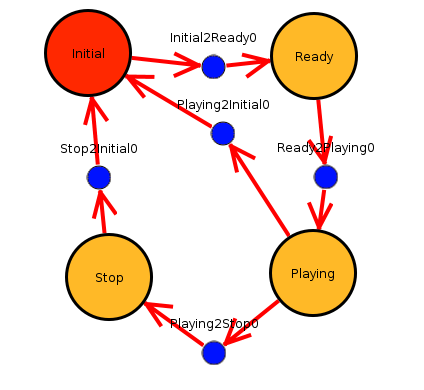
\includegraphics[width=9cm]{img/cap3/estados-music}
  \end{center}
  \caption{M�quina de estados del componente \textbf{Music}.}
  \label{fig:estados-music}
\end{figure}

La m�quina de estados del componente \textbf{Music} la tenemos en la figura \ref{fig:estados-music}. \textit{Initial} es el estado inicial del que se parte cuando se activa el componente. Cuando se carga un fichero, se pasa al estado \textit{Ready}. En este estado el componente est� preparado para empezar a reproducir la m�sica. Cuando se empieza a reproducir el sonido pasamos al estado \textit{Playing}. Por �ltimo, cuando finaliza el fichero de audio, se pasa al estado de \textit{Stop} y de este al estado \textit{Initial}, pero si por el contrario el fichero se para manualmente pasamos al estado \textit{Initial}.\\

\subsection{Componente Body}
\label{subsec:body}

El componente \textbf{Body} se encarga de realizar los movimientos del robot y de caminar. Es modulado por el componente \textbf{Movie} y tambi�n es controlado remotamente desde nuestra aplicaci�n. Los movimientos son fijos y previamente se han creado con una herramienta del JManager. S�lo puede ejecutarse un movimiento a la vez. Hay que tener especial cuidado cuando se ejecuta un movimiento al mismo tiempo que se camina, ya que el movimiento de los brazos puede hacer que el robot pierda el equilibrio y se caiga.\\

\begin{figure} [hbtp]
  \begin{center}
    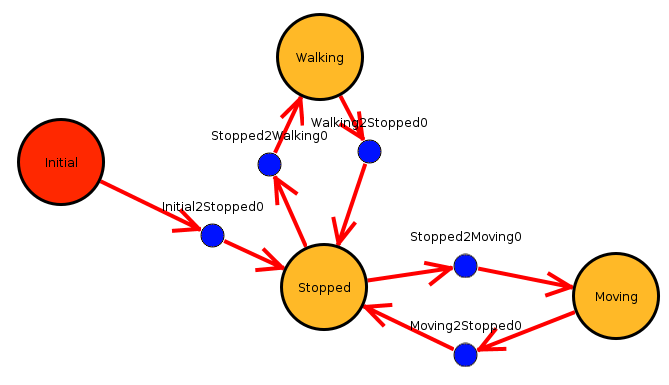
\includegraphics[width=14cm]{img/cap3/estados-body}
  \end{center}
  \caption{M�quina de estados del componente \textbf{Body}.}
  \label{fig:estados-body}
\end{figure}

La m�quina de estados de este componente est� representada en la figura \ref{fig:estados-body}. Cuando se activa el componente, �ste se inicia en el estado \textit{Initial}. En este estado no se hace nada y se avanza directamente al estado \textit{Stopped}. Desde este estado se puede avanzar a los estados \textit{Walking} y \textit{Moving}, dependiendo de c�mo se module. El estado \textit{Walking} se activa cuando el robot comienza a caminar y el estado \textit{Moving}, cuando el robot realiza un movimiento de los que dispone.\\ 

En los estados \textit{Walking} y \textit{Moving} se obliga a pasar por el estado \textit{Stopped}, precisamente para evitar el problema del que hemos hablado al principio de este apartado: evitar caminar y realizar un movimiento al mismo tiempo.

\subsection{Componente Head}
\label{subsec:head}

Este componente es el responsable de mover la cabeza del robot. Tiene dos grados de libertad: pan y tilt. El componente \textbf{Head} contiene m�todos tanto para mover el cuello mec�nico que controla la cabeza como para leer el estado de �ste. Este componente es teleoperado desde  nuestra aplicaci�n.\\

El componente \textbf{Head} no est� formado con una m�quina de estados. Es un componente reactivo, es decir, que responde instant�neamente a las �rdenes que recibe moviendo la cabeza.

\subsection{Componente Movie}
\label{subsec:movie}

El componente \textbf{Movie} fue desarrollado en un Proyecto fin de carrera del grupo de Rob�tica de la universidad, \cite{Benitez2010}. Este componente es el responsable de procesar las sesiones que se siguen en las terapias. Se encarga de recoger informaci�n a partir de un fichero de guiones y activar la ejecuci�n.\\

\begin{figure} [t]
  \begin{center}
    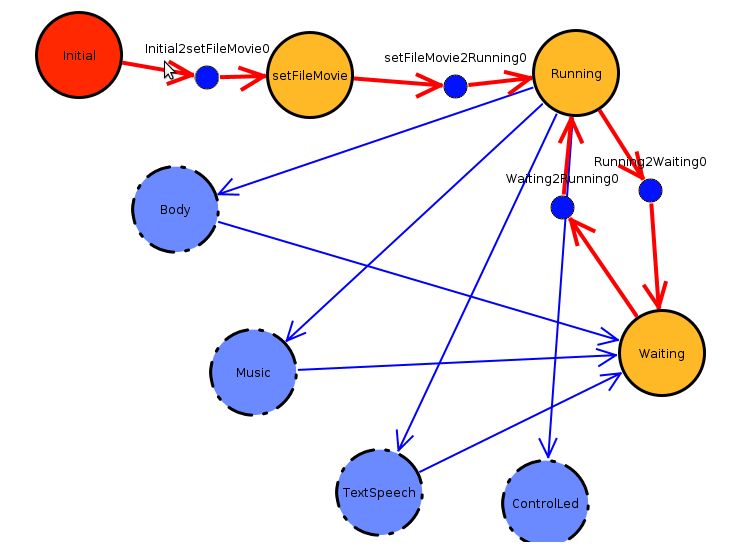
\includegraphics[width=15cm]{img/cap3/estados-movie}
  \end{center}
  \caption{M�quina de estados del componente \textbf{Movie}.}
  \label{fig:estados-movie}
\end{figure}

Como la gran mayor�a de los componentes de BICA, \textbf{Movie} est� formado por una m�quina de estados finita (Figura \ref{fig:estados-movie}). Esta m�quina de estados est� compuesta por cuatro estados. \textit{Initial} es el estado inicial del que se parte cuando se activa el componente. Se pasa al estado \textit{SetFile} cuando se carga una sesi�n. En el estado \textit{Running} se procesa el fichero y se ejecutan los comandos correspondientes. Cuando se encuentra un comando llamado \texttt{wait}, la m�quina de estados avanza al estado \textit{Waiting}. Desde este estado se vuelve al estado \textit{Running} cuando se cumple la condici�n del comando \texttt{wait}.\\

Los componentes con los que interact�a el componente \textbf{Movie} son \textbf{Body}, \textbf{Music}, \textbf{TextSpeech} y \textbf{LedsControl}. De los componentes \textbf{Music} y \textbf{Body} ya hemos hablado en las subsecciones \ref{subsec:music} y \ref{subsec:body} respectivamente. El componente \textbf{TextSpeech} reproduce textos con voz. El componente \textbf{LedsControl} permite controlar los distintos LEDs de los que dispone el robot. Estos dos componentes son modulados �nicamente desde el componente \textbf{Movie}.\\

Los guiones de las terapias est�n escritos en un pseudo-lenguaje creado espec�ficamente para esta tarea. El lenguaje est� compuesto por comandos y los guiones, a su vez, est�n compuestos por una sucesi�n de comandos escritos, uno por cada l�nea del fichero. �stos se ejecutar�n una a una en el orden en que se encuentran en el fichero. A continuaci�n ponemos un peque�o fragmento de una sesi�n que se utiliza actualmente en las terapias y se explica cada una de las l�neas.

\begin{lstlisting}[style=sh] 
mov introduccion
music /home/nao/mp3/vocescien/Clip_sonido_02.mp3
wait task mov
wait task music
wait press left
breakpoint
\end{lstlisting}

\begin{packed_enum}
\item \textbf{mov introduccion - } El robot realiza el movimiento llamado ''introduccion''.
\item \textbf{music /home/nao/mp3/vocescien/Clip\_sonido\_02.mp3 - } Se reproduce el fichero de audio que se encuentra en la ruta \textit{/home/nao/mp3/vocescien/Clip\_sonido\_02.mp3}.
\item \textbf{wait task mov - } El robot espera a que termine el movimiento que est� en ejecuci�n, en este caso es el movimiento ''introduccion'', para seguir con la sesi�n.
\item \textbf{wait task music - } El robot espera a que termine de reproducir el fichero de audio que est� reproduci�ndose, en este caso \textit{/home/nao/mp3/vocescien/Clip\_sonido\_02.mp3}, para ejecutar la siguiente instrucci�n de la sesi�n.
\item \textbf{wait press left - } El robot espera a que se presione el bot�n del pie izquierdo.
\item \textbf{breakpoint - } Se marca un punto de ruptura para poder volver a �l cuando el usuario desee.
\end{packed_enum}

\section{JManager}
\label{sec:jmanager}

JManager es una aplicaci�n de escritorio desarrollada en Java que contiene herramientas para la monitorizaci�n, configuraci�n y depuraci�n del robot. La figura \ref{fig:pantallazos-jmanager} est� compuesta por varias capturas de pantalla de la esta aplicaci�n.\\

\begin{figure}[hbtp]
  \centering
  \begin{tabular}{cc}
  \subfloat[Pantalla de conexi�n.]{
    \label{fig:pantallazo-jmanager}
    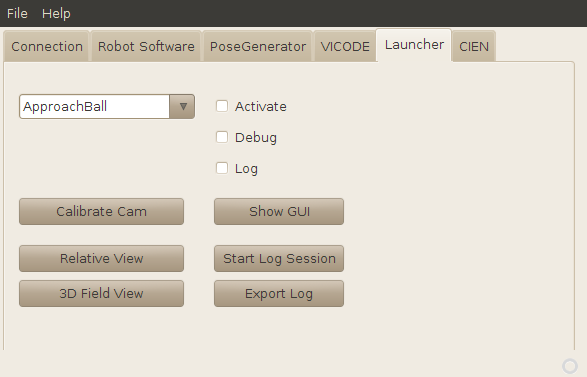
\includegraphics[scale=0.25]{img/cap3/Pantallazo-jmanager}
  } &
    \subfloat[Herramienta de depuraci�n de Vista relativa.]{
    \label{fig:pantallazo-RelativeView}
    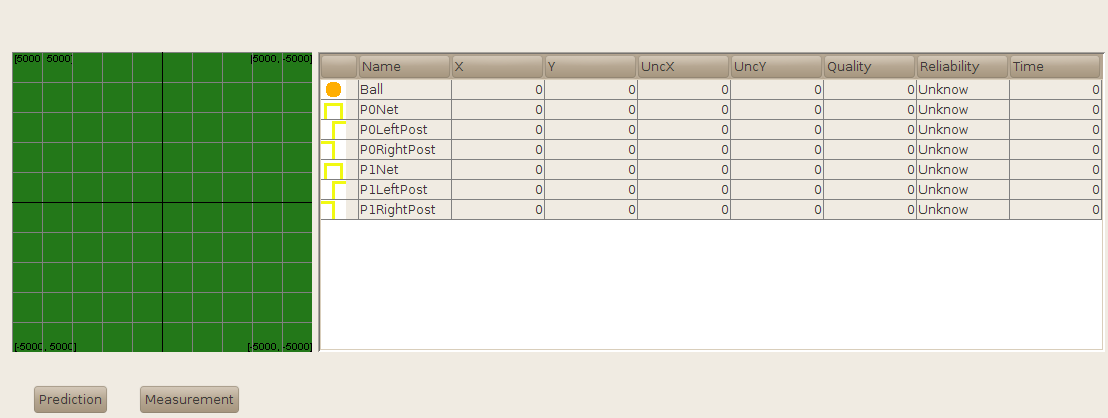
\includegraphics[scale=0.25]{img/cap3/Pantallazo-RelativeView}
  } \\
  \subfloat[Pantalla de activaci�n y desactivaci�n de componentes.]{
    \label{fig:pantallazo-jmanager-1}
    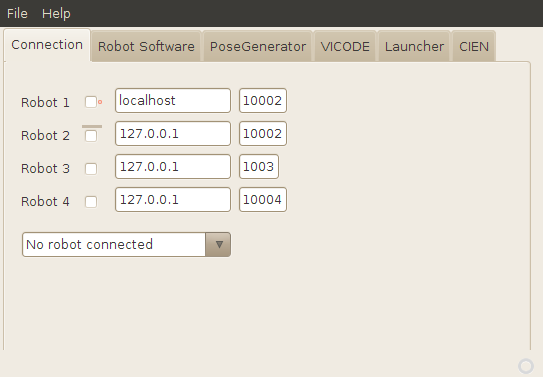
\includegraphics[scale=0.25]{img/cap3/Pantallazo-jmanager-1}
  } &
  \subfloat[Herramienta de depuraci�n de Campo de f�tbol en 3D y configuraci�n del GroundTruth.]{
    \label{fig:pantallazo-3DFieldView}
    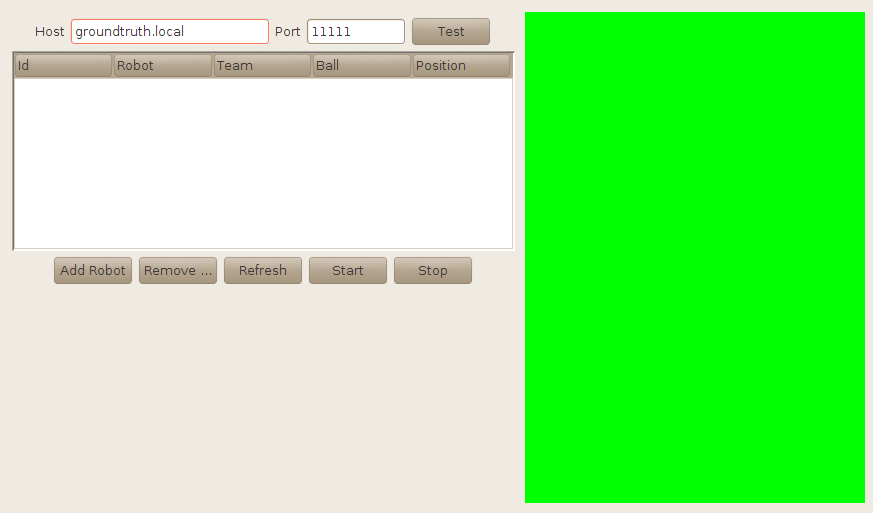
\includegraphics[scale=0.25]{img/cap3/Pantallazo-3DFieldView}
  }
  \end{tabular}
  \caption{Distintas capturas de JManager.}
  \label{fig:pantallazos-jmanager}
\end{figure}

La aplicaci�n JManager est� organizada en varias pesta�as, donde cada una proporciona una funcionalidad distinta. Una de estas funcionalidades es la activaci�n y desactivaci�n de los componentes disponibles en el robot (Figura \ref{fig:pantallazo-jmanager-1}). De igual manera se puede activar el modo de depuraci�n y la interfaz gr�fica propia de cada componente para modularlo y depurarlo. Las figuras \ref{fig:pantallazo-RelativeView} y \ref{fig:pantallazo-3DFieldView} son dos herramientas de depuraci�n que pueden ser usadas por cualquier componente. La primera de estas dos herramientas es muy �til para depurar los algoritmos de localizaci�n de objetos respecto del robot. En el contexto del f�tbol rob�tico se utiliza para depurar la localizaci�n de la pelota, de los jugadores y de las porter�as. La segunda de ellas sirve para configurar la herramienta de GroundTruth y es muy �til para depurar los algoritmos de autolocalizaci�n que se utilizan en el f�tbol rob�tico.\\

Las conexiones con el robot se realizan a trav�s de la red con ayuda de ICE. La figura \ref{fig:jmanager} es un esquema que representa la conexi�n entre JManager con la interfaz de ICE de cada componente.\\

\begin{figure} [hbtp]
  \begin{center}
    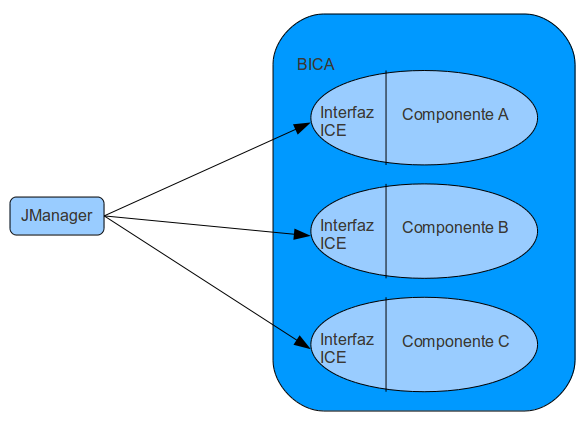
\includegraphics[width=9cm]{img/cap3/jmanager}
  \end{center}
  \caption{Conexi�n entre JManager y BICA.}
  \label{fig:jmanager}
\end{figure}

Otra funcionalidad incluida en el JManager es VICODE, \textit{VIsual COmponent DEsigner}. Se muestra una captura de pantalla de la herramienta en la figura \ref{fig:pantallazo-vicode}. VICODE es una herramienta visual que permite dise�ar componentes BICA. Esta herramienta genera el c�digo C++ de un componente BICA que puede ser integrado directamente dentro de la arquitectura.\\

\begin{figure} [hbtp]
  \begin{center}
    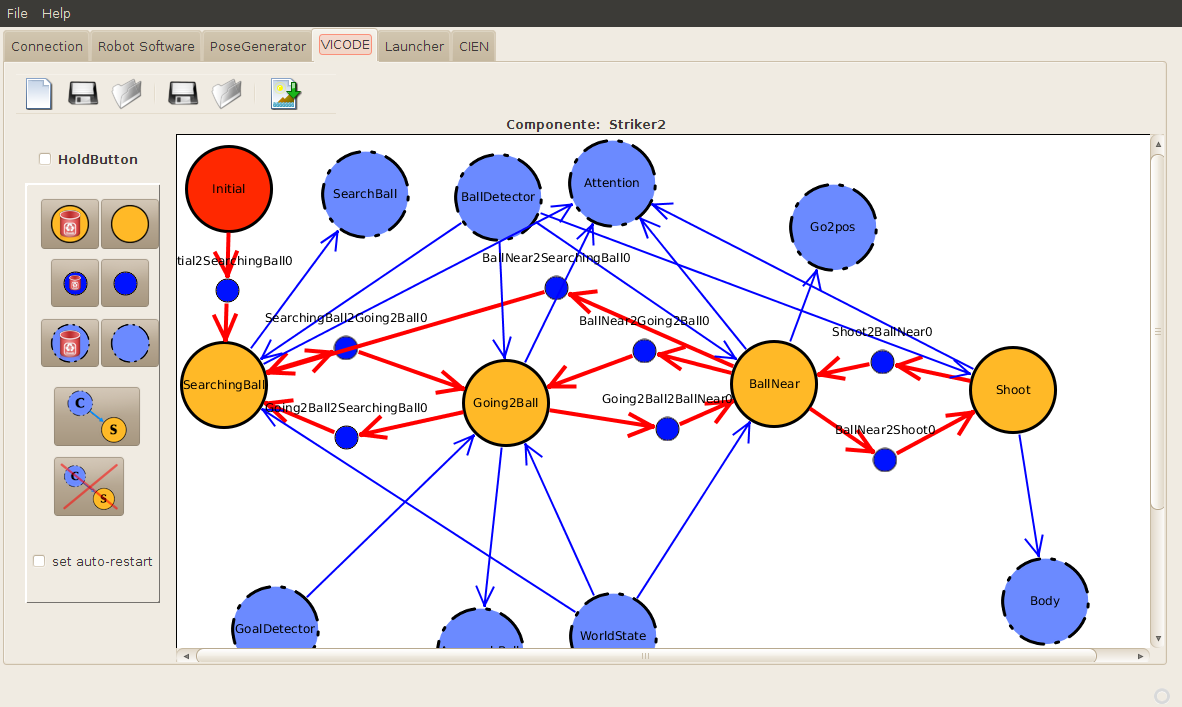
\includegraphics[scale=0.35]{img/cap3/Pantallazo-vicode}
  \end{center}
  \caption{Pantallazo de VICODE.}
  \label{fig:pantallazo-vicode}
\end{figure}

\section{Wiimote} 
\label{sec:wiimote}

Tambi�n conocido como \textbf{Wii Remote} o simplemente \textbf{mando de la Wii}. Es el mando principal de la videoconsola \textit{Wii} de Nintendo. Ambos salieron al mercado a finales de 2006. El Wiimote (Figura \ref{sec:wiimote}) fue dise�ado para utilizarse con una sola mano, en vez de los t�picos mandos de videoconsola que se hab�an creado hasta el momento. Tiene un dise�o parecido al de un mando de televisi�n. Esta caracter�stica aporta al mando mayor intuitividad a la hora de manejarlo, ya que es sensible al movimiento. Con este dise�o, Nintendo quer�a atraer al mundo de los videojuegos a gente que nunca hab�a jugado.\\

El Wiimote es un control remoto inal�mbrico que utiliza la tecnolog�a \textit{bluetooth} para conectarse pudiendo alejarse hasta 10 metros del punto de conexi�n. Dispone de siete botones, uno de ellos con forma de gatillo colocado en la parte posterior del mando. Tambi�n tiene una cruz de direcciones y un bot�n de encendido/apagado. Adem�s, en la parte frontal incorpora un peque�o altavoz y cuatro luces numeradas que indican el n�mero de jugador cuando est� conectado a una Nintendo Wii. La sensibilidad al movimiento la consigue gracias a unos aceler�metros que detectan el movimiento a lo largo de tres ejes. En la parte superior, el mando dispone de una c�mara de infrarrojos que, junto con una barra de LEDs infrarrojos que viene con la videoconsola, convierte el mando en un dispositivo apuntador. Por �ltimo, tambi�n dispone de una memoria de 16KB, de los cuales 6 pueden ser libremente le�dos o escritos, y lleva incorporado un mecanismo vibrador. Como fuente de alimentaci�n utiliza dos bater�as AA, que dotan al mando de una autonom�a de entre 25 y 60 horas, dependiendo de las funcionalidades que se utilicen.

\begin{figure} [hbtp]
  \begin{center}
    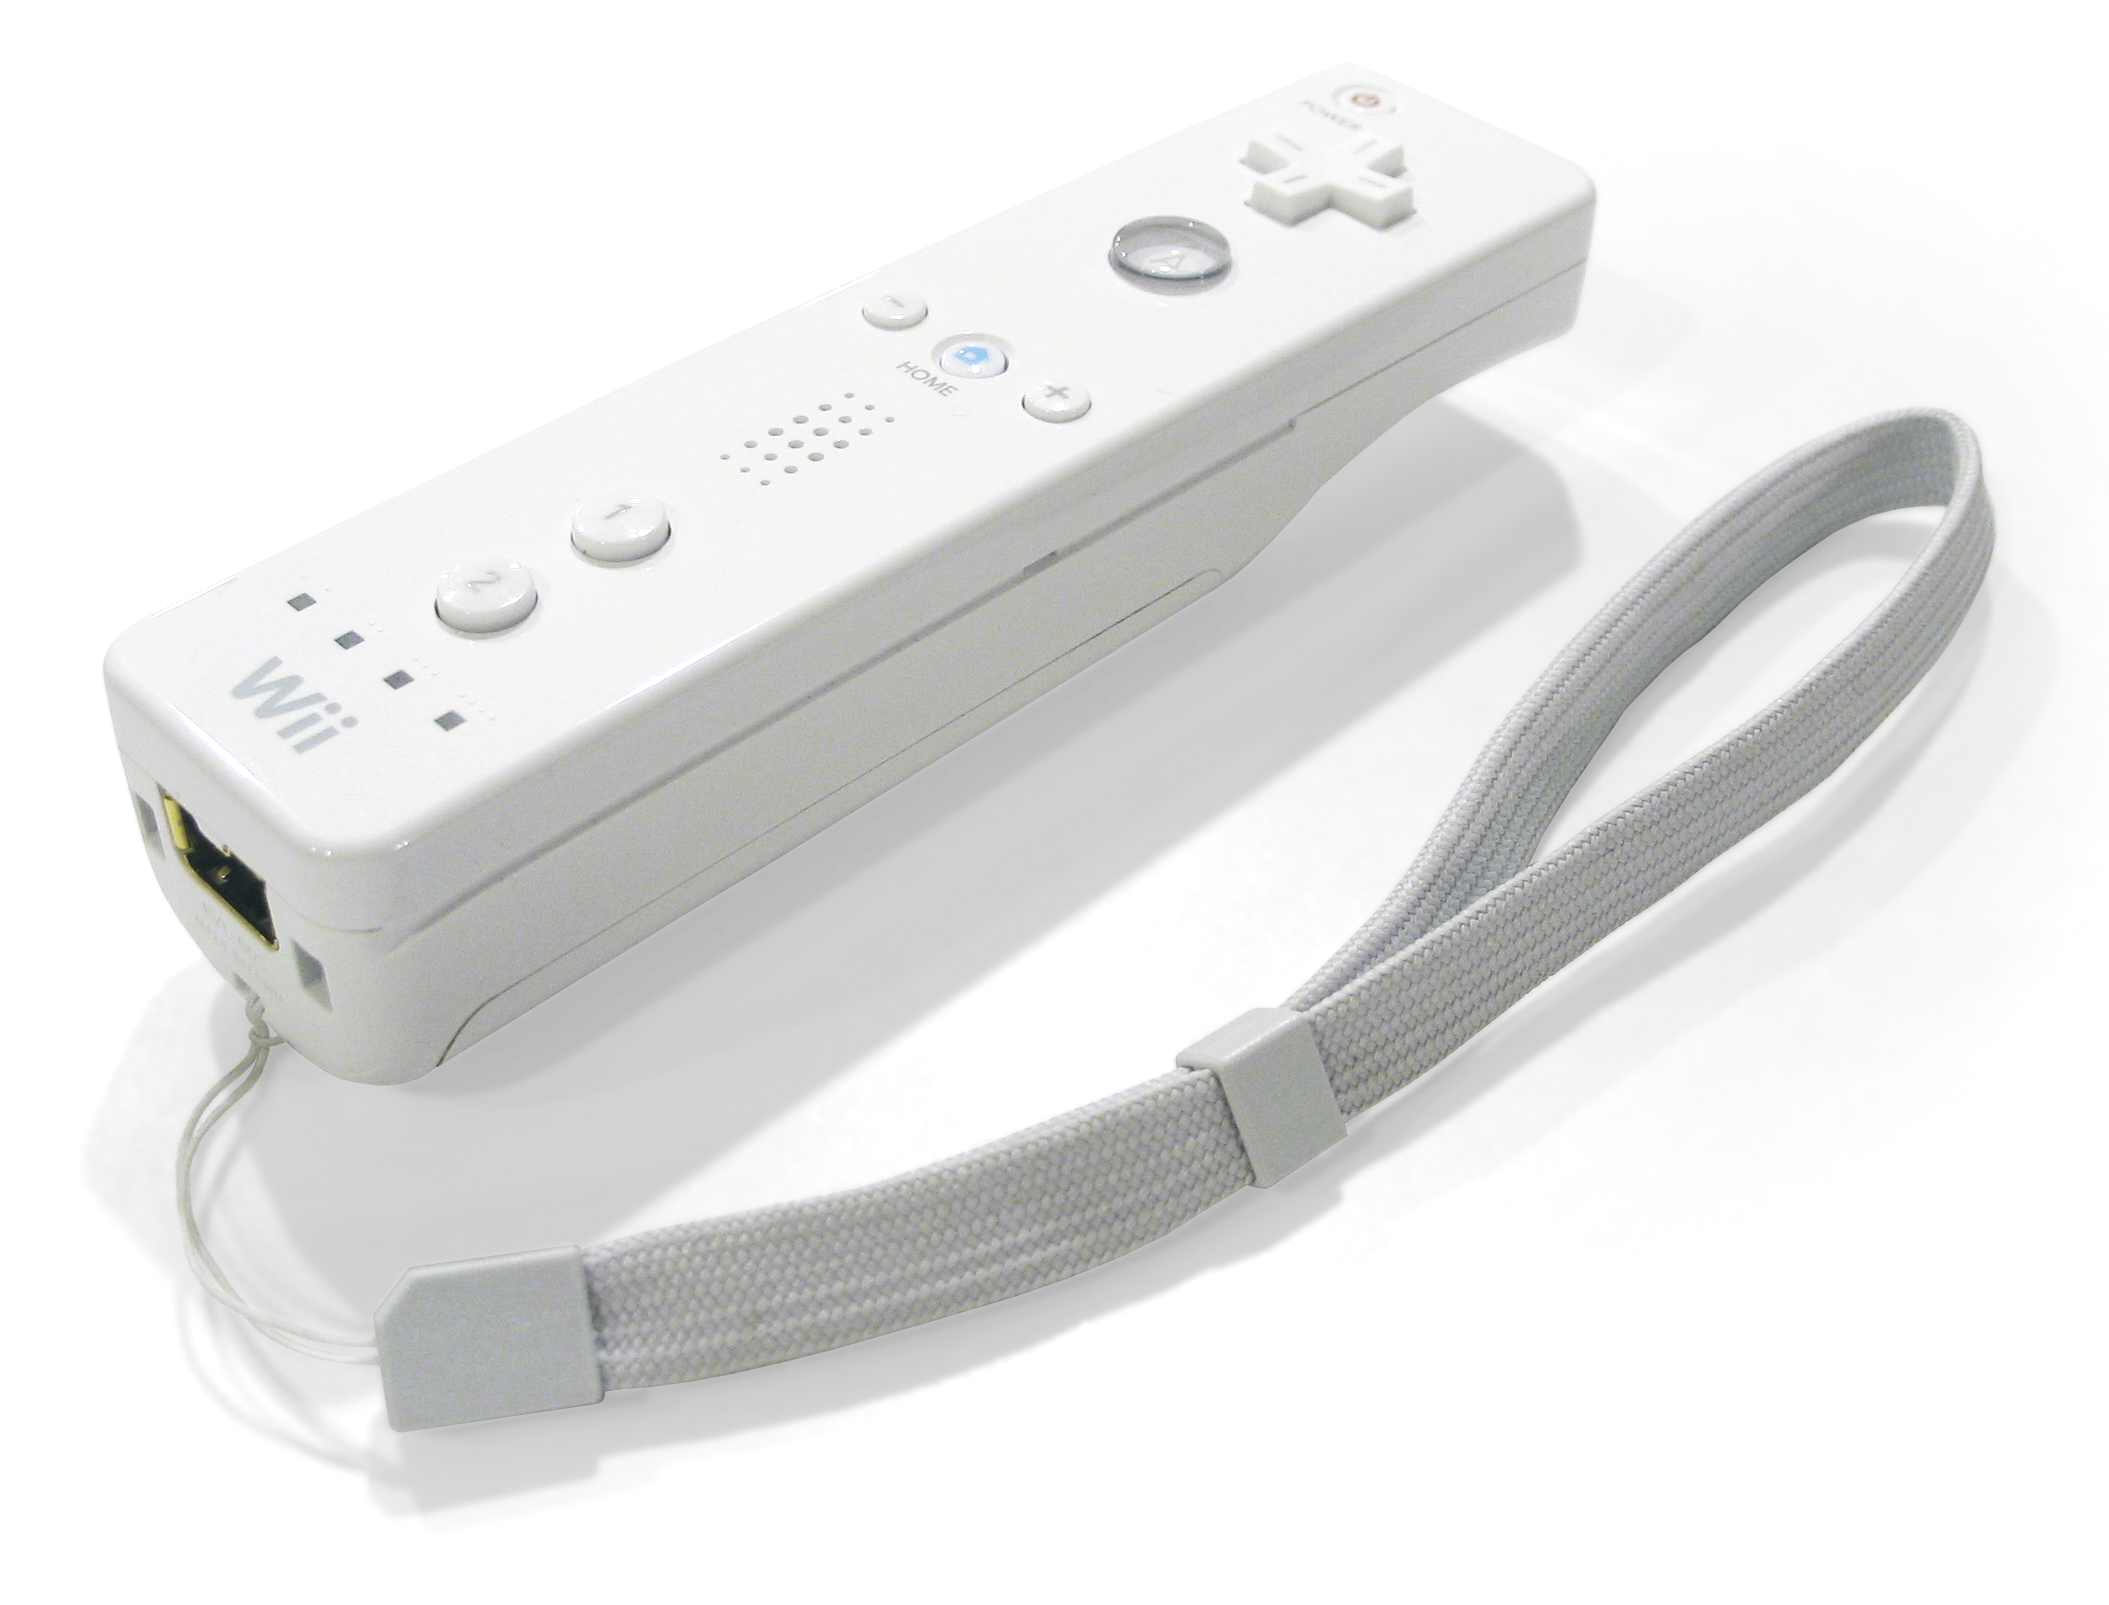
\includegraphics[width=9cm]{img/cap3/wiimote}
  \end{center}
  \caption{Mando de control remoto de la Nintendo Wii, el Wiimote.}
  \label{fig:wiimote}
\end{figure}\

Adem�s de todas las funciones de las que dispone el mando, este dispone de un puerto de expansi�n en su parte inferior que permite a�adir perif�ricos.
Uno de los m�s populares es el \textit{Nunchuk}. Este es un joystick anal�gico con dos botones. Es necesario utilizar la otra mano para manejarlo. Existen muchos otros perif�ricos que se pueden utilizar con el mando, pero que s�lo son �tiles para jugar a algunos videojuegos y no para nuestra investigaci�n, por lo que no hablaremos de ellos.\\

Hemos escogido este dispositivo de control auxiliar porque cumple con todos los requisitos que se hab�an propuesto. Es un dispositivo dise�ado para que sea f�cil de utilizar para gente que no est� acostumbrada a usar este tipo de controles. Que se pueda utilizar con una sola mano junto con que sea inal�mbrico, aporta a la terapeuta mayor autonom�a y le da la posibilidad de poder moverse por la sala e interactuar con los pacientes.\\

Para implementar este dispositivo se ha utilizado una biblioteca externa de software libre, \textit{Motej v0.9}. Esta biblioteca est� publicada bajo la licencia de Apache \textit{ASL 2.0}\footnote{http://www.apache.org/licenses/LICENSE-2.0.html}. \textit{Motej} es una biblioteca Java de comunicaci�n con el Wiimote. Permite controlar distintos aspectos del mando como la lectura de los aceler�metros, el control de vibraci�n, el encendido y apagado de los LEDs, la lectura de los botones y de la memoria EEPROM, la escritura de los registros del mando, la informaci�n de estado y los datos de calibraci�n.












% Capitulo 4
\chapter{Descripci�n inform�tica}
\label{cap:descripcion}

En este cap�tulo se detalla el trabajo realizado dentro de este proyecto. Se hablar� de las mejoras introducidas en la realizaci�n de las terapias y de las herramientas creadas.

\begin{figure} [hbtp]
  \begin{center}
    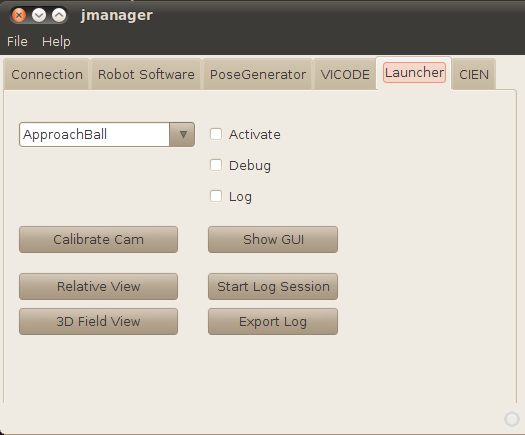
\includegraphics[width=9cm]{img/cap4/componentes-jmanager}
  \end{center}
  \caption{Captura de pantalla de la pesta�a de administraci�n de los \textit{componentes} en la herramienta JManager.}
  \label{fig:componentes-jmanager}
\end{figure}

El trabajo no se limita �nicamente a las herramientas desarrolladas, sino que la experimentaci�n y la realimentaci�n son aspectos clave en el trabajo realizado. En primer lugar se eval�a el estado tecnol�gico en el que se encuentran las herramientas utilizadas en las sesiones de Roboterapia. Para ello se acudi� a varias terapias, para comprender bien el contexto del problema y las necesidades reales de los terapeutas cuando est�n trabajando. Despu�s se describir� la aplicaci�n de escritorio creada para la realizaci�n las terapias. Tambi�n se explicar� c�mo se ha integrado el Wiimote con la aplicaci�n y c�mo se usa. Por �ltimo, se explican las sesiones que se han implementado para poder realizar las terapias con nuevos grupos.

\section{Evaluaci�n del estado de las herramientas disponibles}
\label{sec:evaluacion}

Las sesiones de Roboterapia estaban realiz�ndose con las herramientas creadas por Ra�l Ben�tez Mej�a, \cite{Benitez2010}. Estas herramientas estaban integradas en el JManager, aplicaci�n de la cual hemos hablado en \ref{sec:jmanager}. Siguiendo la filosof�a de componentes de BICA, el JManager dispone de una interfaz gr�fica para modular cada componente. Primero es necesario activar manualmente los componentes que se quieren utilizar. En nuestro caso se deben activar los componentes de los que se ha hablado en el cap�tulo anterior: \textbf{Body}, \textbf{Head}, \textbf{Music} y \textbf{Movie}. La figura \ref{fig:componentes-jmanager} es una captura de pantalla de la pesta�a de la herramienta JManager en la que se activan y desactivan los \textit{componentes} de BICA. Adem�s de esta funcionalidad tiene otras, como pueden ser la activaci�n del modo de depuraci�n de los \textit{componentes} o la activaci�n de distintas herramientas de depuraci�n del JManager.\\

Una vez que los \textit{componentes} est�n activos, seleccionando cada uno de ellos, hay que pulsar sobre el bot�n con el t�tulo \textit{Show GUI} para mostrar la interfaz gr�fica con la que modular dicho \textit{componente} (Figura \ref{fig:conexion-jmanager-bica}). Estas interfaces fueron creadas para probar, depurar y utilizar los \textit{componentes}, pero de manera individual y sin un contexto determinado. En un contexto como el que se presenta, las terapias, dichas interfaces son inc�modas y, en ocasiones, dif�ciles de usar. Tambi�n resulta complicado teleoperar al robot al tiempo que se realiza una sesi�n con tantas ventanas abiertas.

\begin{figure} [hbtp]
  \begin{center}
    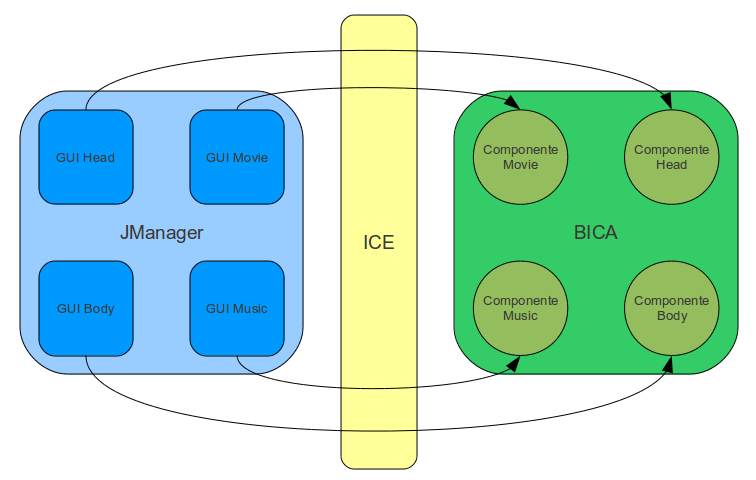
\includegraphics[width=12cm]{img/cap4/conexion-jmanager-bica}
  \end{center}
  \caption{Esquema de modulaci�n de un \textit{componente} desde el GUI correspondiente.}
  \label{fig:conexion-jmanager-bica}
\end{figure}

Antes de empezar a dise�ar e implementar la aplicaci�n, es imprescindible evaluar en profundidad las herramientas que hay disponibles y descubrir los aspectos en los que fallan durante una terapia.
A continuaci�n se analiza por separado cada una de las interfaces gr�ficas de los \textit{componentes} BICA y se resaltar�n los puntos negativos.

\subsection{Evaluaci�n del componente Music}
\label{subsec:analisis-music}

En la figura \ref{fig:captura-music} se muestra una captura de pantalla de la interfaz gr�fica del componente \textbf{Music}. Este \textit{componente} es bastante sencillo de utilizar. Para reproducir un fichero se introduce en el campo de texto disponible la ruta de dicho fichero. Esta ruta debe ser absoluta y representa donde se ubica el fichero, pero en el sistema de ficheros del robot, no de la m�quina donde se ejecuta el JManager. Despu�s se carga el fichero mediante el bot�n \textit{Load MP3} y se reproduce con el bot�n \textit{Play}. La reproducci�n se puede parar en cualquier momento pulsando \textit{Stop}. Mediante el slider del inferior de la ventana se regula el volumen.

\begin{figure} [hbtp]
  \begin{center}
    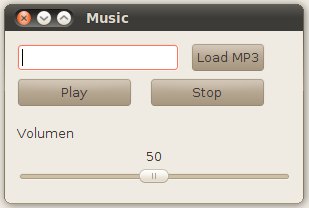
\includegraphics[width=6cm]{img/cap4/captura-music}
  \end{center}
  \caption{Captura de pantalla de la interfaz gr�fica del componente \textbf{Music}.}
  \label{fig:captura-music}
\end{figure}

Este m�todo de reproducir ficheros es bastante inc�modo. Los inconvenientes que tiene son:

\begin{enumerate}
\item Es necesario conocer la ruta exacta de d�nde se encuentra el fichero que se quiere reproducir en el sistema de ficheros remoto, el del robot. 
\item Para reproducir un fichero hay que hacer demasiadas acciones. Primero hay que introducir la ruta del fichero, segundo pulsar \textit{Load MP3} y, por �ltimo, pulsar \textit{Play} para que suene. 
\end{enumerate}


\subsection{Evaluaci�n del componente Body}
\label{subsec:analisis-body}

En la figura \ref{fig:captura-body} se muestra una captura de pantalla de la interfaz gr�fica del componente \textbf{Body}. Desde ella se puede teleoperar al robot y hacer que se desplace. Mediante los sliders se ajusta la velocidad de la caminata. Cada uno de ellos ajusta un par�metro: la velocidad lineal, la de rotaci�n y la de desplazamiento lateral. Cuando se que quiere para se pulsa el bot�n de \textit{Stop}.  Para ejecutar los movimientos fijos disponibles en el robot, se utiliza el campo de texto de la esquina superior derecha. En �l se introduce el nombre del movimiento y se pulsa el bot�n \textit{doMove}. Los botones de la esquina inferior derecha son movimientos de distintas patadas que utiliza el robot cuando juega al f�tbol para golpear la pelota. Esta interfaz presenta varios inconvenientes:


\begin{figure} [hbtp]
  \begin{center}
    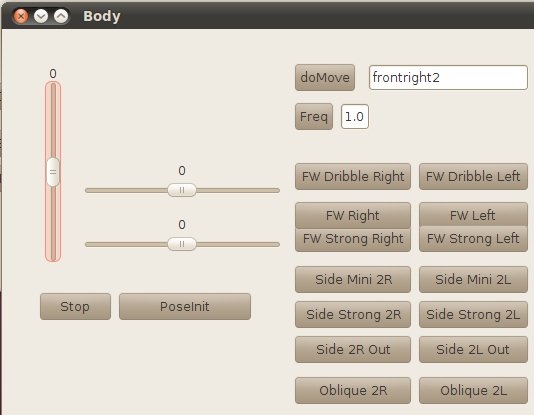
\includegraphics[width=9cm]{img/cap4/captura-body}
  \end{center}
  \caption{Captura de pantalla de la interfaz gr�fica del componente \textbf{Body}.}
  \label{fig:captura-body}
\end{figure}

\begin{enumerate}
\item No se sabe qu� slider ajusta qu� par�metro de la caminata. Se puede intuir que el vertical ajusta la velocidad lineal del robot, pero los otros dos, los que ajustan la velocidad de rotaci�n y la lateral, no se distinguen.
\item Los sliders est�n implementados seg�n el sistema de coordenadas que utiliza el robot. Como �ste utiliza un sistema de coordenadas dextr�giro cuando el valor del slider crece, se acerca al extremo derecho, el robot gira a la izquierda, mientras que si decrece, se acerca al extremo izquierdo, el robot gira a la derecha. Este sistema es antiintuitivo y hace dif�cil controlar al robot con precisi�n. En la imagen se puede ver el eje de coordenadas del robot superpuesto en la imagen.

\begin{figure} [hbtp]
  \begin{center}
    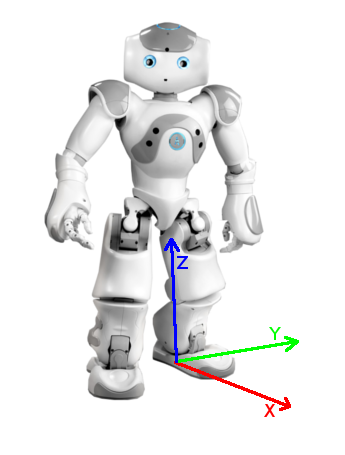
\includegraphics[width=8cm]{img/cap4/sistema-coordenadas-robot}
  \end{center}
  \caption{Sistema de coordenadas dextr�giro.}
  \label{fig:sistema-coordenadas-robot}
\end{figure}

\item Los botones de la esquina inferior derecha, que ejecutan distintas patadas, son irrelevantes para las terapias. Son muy �tiles en el contexto del f�tbol rob�tico, pero in�tiles en el de las sesiones de Roboterapia.
\item Al igual que pasaba con la reproducci�n de los ficheros de audio, el m�todo para ejecutar movimientos fijos es inc�modo. Es necesario saberse el nombre del movimiento, escribirlo y luego pulsar el bot�n \textit{doMove}. Demasiadas acciones para ejecutar un s�lo movimiento.
\end{enumerate}

\subsection{Evaluaci�n del componente Head}
\label{subsec:analisis-head}

En la figura \ref{fig:captura-head} se muestra una captura de pantalla de la interfaz gr�fica del componente \textbf{Head}. Esta interfaz dispone de dos m�todos de control de la cabeza. Uno es modulando la velocidad y posici�n del cuello mec�nico y otro, modulando solamente la velocidad. Mediante los sliders se ajusta dicha posici�n o la velocidad de movimiento del cuello. El slider horizontal modula el par�metro Pan y el vertical, el Tilt. Mediante el bot�n situado arriba a la izquierda se cambia de un modo a otro.\\

Esta interfaz es bastante sencilla de utilizar, aunque presenta un inconveniente: en ocasiones no queda claro cu�l de los dos m�todos se est� usando. Es necesario fijarse en el bot�n superior izquierdo para saberlo, lo cual resulta inc�modo cuando se est� pendiente de llevar la terapia m�s que de teleoperar al robot.

\begin{figure} [hbtp]
  \begin{center}
    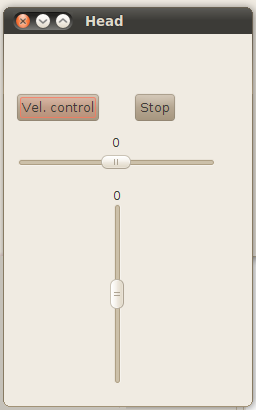
\includegraphics[width=5cm]{img/cap4/captura-head}
  \end{center}
  \caption{Captura de pantalla de la interfaz gr�fica del componente \textbf{Head}.}
  \label{fig:captura-head}
\end{figure}

\subsection{Evaluaci�n del componente Movie}
\label{subsec:analisis-movie}

Por �ltimo, la figura \ref{fig:captura-movie} muestra una captura de pantalla de la interfaz gr�fica del componente \textbf{Movie}. Este \textit{componente} es bastante m�s complejo de utilizar que los otros. Esto es l�gico, ya que este \textit{componente} contiene m�s funcionalidades.\\

Mediante el bot�n \textit{Load Movie} aparece un di�logo para seleccionar la sesi�n que se quiere abrir. El bot�n \textit{Create Movie} sirve para crear un gui�n. Mediante los bot�nes \textit{Pause}, \textit{Play} y \textit{Stop} se puede pausar, reanudar o parar el gui�n que se est� reproduciendo. Los botones \textit{Previous BreakPoint} y \textit{Next BreakPoint} sirven para buscar autom�ticamente en el fichero el breakpoint siguiente y el anterior. El gui�n cargado se muestra en el �rea de texto del centro de la ventana. Mediante los botones situados justo debajo de este �rea de texto se puede salvar el fichero si se edita con el bot�n \textit{Save} o enviarlo al robot, mediante el bot�n \textit{Send File to Robot}. El �rea de texto de la derecha contiene informaci�n sobre los comandos que se pueden utilizar en los guiones.\\

\begin{figure} [hbtp]
  \begin{center}
    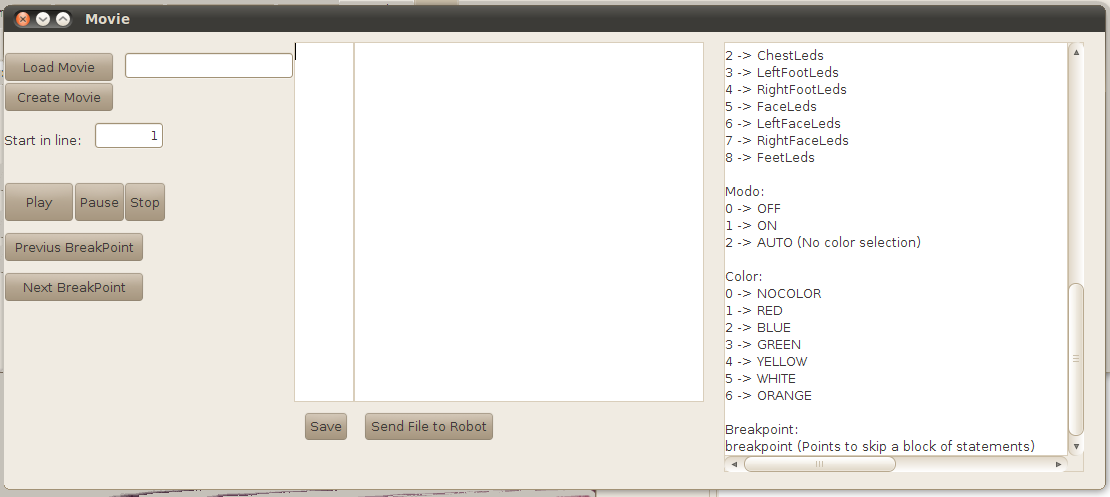
\includegraphics[width=15cm]{img/cap4/captura-movie}
  \end{center}
  \caption{Captura de pantalla de la interfaz gr�fica del componente \textbf{Movie}.}
  \label{fig:captura-movie}
\end{figure}

Este interfaz gr�fico contiene mucha funcionalidad, lo que provoca que sea confuso y dif�cil de manejar. Los inconvenientes que presenta son:

\begin{enumerate}
\item El primero y m�s importante es el haber juntado dos funcionalidades bastante complejas en una sola ventana: la edici�n y la ejecuci�n de guiones. Son tantas las cosas que se pueden hacer, que la interfaz resulta confusa y complicada de manejar.
\item Cuando se carga un fichero, para que �ste pueda reproducirse en el robot, deben tener la mismo ruta en ambos sistemas de fichero. Es decir, si en el ordenador donde estamos ejecutando el JManager cargamos el fichero de la ruta \texttt{/home/nao/movies/sesion.movie}, en el robot tambi�n debe existir este mismo fichero con la misma ruta. Esto nos obliga a tener un conocimiento profundo del sistema de ficheros del robot.
\item El uso de los breakpoints es bastante aparatoso y complicado de usar. En caso de que se apague el robot por falta de bater�a o por cualquier otro problema, es dif�cil recuperar el punto donde se qued� la sesi�n.
\item Mostrar los comandos del gui�n no aporta nada a los terapeutas, ya que es dif�cil de leer cuando se ejecuta una sesi�n.
\item En caso de no editar el gui�n, la informaci�n disponible en �rea de texto de la derecha no es necesaria.
\end{enumerate}

Todos los inconvenientes de los distintos \textit{componentes} se han tenido en cuenta para realizar nuestra aplicaci�n y se ha intentado mejorar la usabilidad de �sta.

\section{Aplicaci�n CIEN}
\label{sec:appcien}

Una vez descritos los inconvenientes de la aplicaci�n anterior, en este proyecto se ha desarrollado una aplicaci�n que permita realizar terapias para enfermos de Alzheimer con el robot Nao. Esta aplicaci�n ha de ser sencilla e intuitiva para que sea utilizada por los terapeutas que realizan las terapias. El software creado para dicho fin se presenta en esta secci�n, la Aplicaci�n CIEN.\\

\begin{figure} [hbtp]
  \begin{center}
    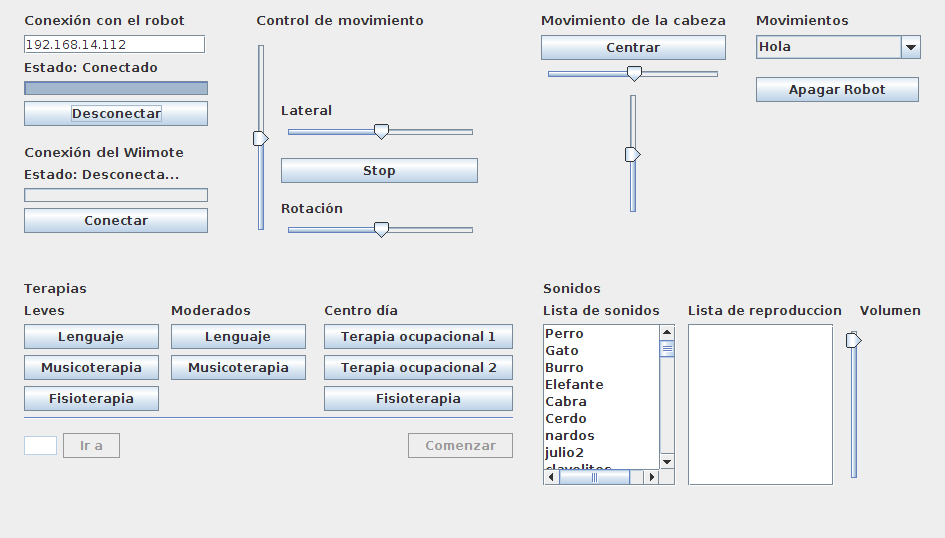
\includegraphics[width=15cm]{img/cap4/captura-cien}
  \end{center}
  \caption{Captura de pantalla de la Aplicaci�n CIEN.}
  \label{fig:captura-cien}
\end{figure}

Como se ha comentado en el cap�tulo \ref{cap:objetivos}, esta aplicaci�n ha sido creada a base de distintos prototipos que eran probados en las terapias. La realimentaci�n para hacer el siguiente prototipo proven�a principalmente de los terapeutas e investigadores encargados de las terapias y de la experiencia personal. La figura \ref{fig:captura-cien} es una captura de pantalla de la interfaz gr�fica de la aplicaci�n. Este es el resultado al que se ha llegado despu�s de numerosas iteraciones.\\

Para hacer lo m�s sencilla posible la aplicaci�n, se optado por agrupar toda la funcionalidad necesaria para las terapias en una sola ventana. Para evitar que la aplicaci�n sea confusa, las distintas funcionalidades se han dividido en peque�os m�dulos, que son: Conexi�n con el robot, Conexi�n del Wiimote, Control de movimiento, Movimiento de la cabeza, Movimientos, Terapias, Sonidos y un bot�n para apagar el robot. Cada uno de estos m�dulos es responsable de una funcionalidad. En las siguientes secciones se expone cada una de estas funcionalidades.

\subsection{M�dulo de conexi�n con el robot}
\label{subsec:conexionrobot}

El m�dulo de conexi�n con el robot (Figura \ref{fig:captura-cien-conexionrobot}), se encarga de gestionar la conexi�n por red con el robot. Dispone de un campo de texto en donde se introduce la direcci�n del robot. El estado de la conexi�n se puede ver por medio de una etiqueta y una barra de progreso. Tambi�n dispone de un bot�n multifunci�n que, dependiendo del estado en el que se encuentra la conexi�n, sirve para conectarse o desconectarse.

\begin{figure} [hbtp]
  \begin{center}
    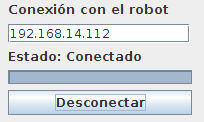
\includegraphics[scale=0.75]{img/cap4/captura-cien-conexionrobot}
  \end{center}
  \caption{Captura de pantalla del m�dulo de conexi�n con el robot.}
  \label{fig:captura-cien-conexionrobot}
\end{figure}

La direcci�n del robot puede introducirse de dos maneras: a trav�s de su ip o a trav�s del nombre del robot junto con el dominio \texttt{.local}. El puerto que utiliza BICA no es necesario conocerlo, la aplicaci�n lo pone autom�ticamente. Para averiguar el n�mero de puerto se sigue la norma de sumar el �ltimo n�mero de la direcci�n ip del robot a 10.000, es decir, si la ip del robot termina en 112, se suma 2 a 10.000, por lo que el puerto de conexi�n es el 10.002.\\

Se ha simplificado al m�ximo la conexi�n con el robot eliminando t�rminos t�cnicos inform�ticos como ip y puerto. Simplemente conociendo el nombre del robot y agregando el dominio \texttt{.local}, el terapeuta que lo utilice puede conectarse a �l, la resoluci�n del nombre se hace autom�ticamente gracias a las bibliotecas de \textit{Avahi}. Esta biblioteca ofrece, entre otros servicios, un servicio de \textit{multicast DNS} para la resoluci�n de nombre en redes de �rea local.\\

Respecto al m�todo de conexi�n con el que se contaba antes, se ha simplificado el proceso. Los t�rminos ip y puerto son b�sicos en �rea de redes inform�ticas, pero pueden confundir a un usuario sin conocimientos inform�ticos. Con este m�todo que se acaba de explicar se simplifica la conexi�n con el robot.

\subsection{M�dulo de conexi�n con el Wiimote}
\label{subsec:conexionwiimote}

El m�dulo de conexion con el Wiimote (Figura \ref{fig:captura-cien-conexionwiimote}), funciona de forma parecida al m�dulo de conexi�n con el robot. El estado de la conexi�n se muestra a trav�s de una etiqueta y de una barra de progreso. S�lo se dispone un bot�n que, dependiendo del estado en el que se encuentra la conexi�n con el Wiimote, sirve para conectarse o desconectarse.\\

\begin{figure} [hbtp]
  \begin{center}
    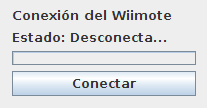
\includegraphics[scale=0.75]{img/cap4/captura-cien-conexionwiimote}
  \end{center}
  \caption{Captura de pantalla del m�dulos de conexion del Wiimote.}
  \label{fig:captura-cien-conexionwiimote}
\end{figure}

Cuando se pulsa el bot�n de conectar, la aplicaci�n inicia una b�squeda a trav�s del bluetooth de los mandos disponibles. Para conectar el mando es necesario pulsar simult�neamente los botones 1 y 2. Los LEDs del mando se pondr�n a parpadear mientras se sincronizan los dispositivos. Si se establece la conexi�n con �xito, el mando vibra y se queda iluminado el primer LED de �ste.\\

Este componente gr�fico es genuino del desarrollo que se ha realizado en este proyecto. Anteriormente, no exist�a ning�n componente que permitiese teleoperar al robot con el Wiimote.

\subsection{M�dulo de control de movimientos del cuerpo}
\label{subsec:movimientoscuerpo}

El m�dulo de control de movimientos del cuerpo est� dividido en dos. Por un lado tenemos un teleoperador para mover al robot (Figura \ref{fig:captura-cien-body}) y, por el otro, un selector de movimientos. El teleoperador est� compuesto por tres sliders que controlan cada uno de los posibles desplazamientos del robot: adelante/atr�s, rotar a un lado y al otro, y el desplazamiento lateral. Tambi�n dispone de un bot�n de parada. El selector de movimientos est� compuesto por una �nica lista desplegable con los movimientos disponibles.\\

\begin{figure}[hbtp]
  \centering
  \subfloat[Teleoperador del robot.]{
    \label{fig:captura-cien-body}
    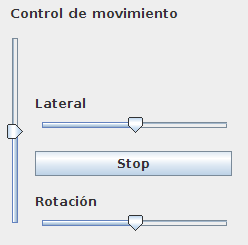
\includegraphics[scale=0.75]{img/cap4/captura-cien-body}
  }
  \subfloat[Selector de movimientos.]{
    \label{fig:captura-cien-movimientos}
    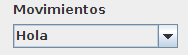
\includegraphics[scale=0.75]{img/cap4/captura-cien-movimientos}
  }
  \caption{Capturas de pantalla de los m�dulos de control de movimientos del cuerpo.}
  \label{fig:movimientoscuerpo}
\end{figure}

Para teleoperar al robot se utilizan los sliders. �stos regulan la velocidad a la que se ejecuta el desplazamiento, cuanto m�s al extremo, m�s r�pido se mover� el robot. Los sliders pueden utilizarse conjuntamente.\\

El selector de movimientos es configurable a trav�s de un fichero de texto. Este se encuentra en el directorio \texttt{conf} del proyecto y se llama \texttt{movements.conf}. La sintaxis del fichero es muy sencilla. Las l�neas que comienzan con ''\#'' se consideran comentarios y los nombres de los movimientos se escribir�n uno en cada l�nea. Esto hace que insertar y eliminar movimientos de la aplicaci�n sea una tarea sencilla. Tambi�n permite poder ver todos los movimientos de un vistazo y elegir el m�s conveniente para la acci�n que se quiera realizar. A continuaci�n se muestra un fragmento de un fichero de configuraci�n.

\begin{lstlisting}[style=sh, numbers=none] 
# Fichero de configuraci�n del m�dulo de movimientos.
# -----------------------------------------------------
# Las l�neas que comienzan con un # se consideran comentarios.
Hola
Adios
Flamenco
Introduccion
\end{lstlisting}

Esta nueva interfaz gr�fica para teleoperar el desplazamiento del robot es m�s intuitiva, ya que se ha seguido el criterio de girar, o desplazarse en el caso del movimiento lateral, hacia el mismo lado que se mueve el slider. Es decir, si se desplaza el slider a la derecha, el robot gira o se desplaza a la derecha. Por otro lado, se ha mejorado y facilitado el acceso a los movimientos que puede realizar el robot, mostrando los disponibles en un men� desplegable. Esto evita tener que conocer el nombre de los movimientos que puede ejecutar el robot. Para reproducir un movimiento simplemente hay que seleccionarlo.

\subsection{M�dulo de control de movimientos de la cabeza}
\label{subsec:movimientoscabeza}

El m�dulo de control de los movimientos de la cabeza (Figura \ref{fig:captura-cien-cabeza}) permite teleoperar el cuello del robot y hacer que \textit{mire} a los pacientes. Poder dirigir la mirada del robot a los pacientes y establecer un contacto visual, ayuda al robot a integrarse en mayor medida con los pacientes de las terapias y les incita a participar. La comunicaci�n con contacto visual siempre es m�s natural. Se maneja con dos sliders, uno sirve para ajustar el movimiento horizontal y el otro para ajustar el movimiento vertical. Adem�s, dispone de un bot�n para centrar la cabeza.\\

\begin{figure} [hbtp]
  \begin{center}
    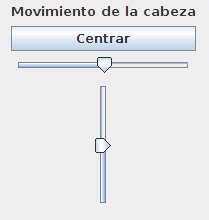
\includegraphics[scale=0.75]{img/cap4/captura-cien-cabeza}
  \end{center}
  \caption{Captura de pantalla del m�dulo de control de la cabeza.}
  \label{fig:captura-cien-cabeza}
\end{figure}

La posici�n donde se encuentra el slider indica la posici�n de la cabeza, coincidiendo la posici�n m�xima del slider con la posici�n m�xima de la cabeza. Se ha preferido implementar uno s�lo de los dos m�todos de control de la cabeza para que la tarea sea m�s sencilla y no complicar las cosas a la terapeuta.

\subsection{M�dulo de control de terapias}
\label{subsec:terapias}

El m�dulo de control de las terapias (Figura \ref{fig:captura-cien-terapias}) se encarga de ejecutar los guiones de las terapias. Esta formado por unos botones con los que se cargan las terapias, un bot�n para ejecutar la siguiente acci�n de la terapia y otro para seleccionar una l�nea concreta del gui�n y ejecutarla directamente.\\

\begin{figure} [hbtp]
  \begin{center}
    \includegraphics[scale=0.75]{img/cap4/captura-cien-terapias}
  \end{center}
  \caption{Captura de pantalla del m�dulo de control de las terapias.}
  \label{fig:captura-cien-terapias}
\end{figure}

Para usar este m�dulo, lo primero es cargar una terapia mediante el bot�n correspondiente. Una vez cargada la terapia, se habilitan los botones situados en la parte inferior. El bot�n situado a la derecha es el que m�s se utiliza. Sirve para comenzar la terapia y para continuar la siguiente acci�n, cuando el robot efect�a una pausa. El campo de texto situado a la izquierda sirve para introducir el n�mero de l�nea que quieres ejecutar y con el bot�n \textit{Ir a} se inicia la acci�n.\\

La funci�n de poder escoger el n�mero de l�nea que se quiere ejecutar es muy �til cuando se quieren hacer saltos en la sesi�n. Normalmente, los guiones se ejecutan enteros, pero en ocasiones, por falta de tiempo, se acortan. Tambi�n es muy �til cuando ocurre alg�n problema con el robot. El m�s habitual es que se agote la bater�a. En estos casos se puede retomar la sesi�n donde se qued�.\\

En un principio, para poder ejecutar el siguiente comando de un gui�n hab�a que pulsar siempre el bot�n situado en la punta del pie izquierdo. Esto era inc�modo y tedioso para el terapeuta, ya que le obligaba a estar cerca del robot para poder pulsar el bot�n y continuar con la terapia. Esta funcionalidad se ha mantenido, pero gracias al bot�n de \textit{Siguiente} se puede ejecutar el comando siguiente sin necesidad de pulsar el bot�n del pie. Esto aporta al terapeuta mayor autonom�a y facilita la interacci�n con los pacientes, ya que puede moverse por todo el aula.\\

Respecto al interfaz anterior se ha implementado solamente la funcionalidad de reproducir guiones. Un terapeuta que est� realizando una sesi�n no puede ponerse a editar el gui�n, porque no puede desatender a los pacientes. En caso de que haya necesidad de modificar un gui�n, se hace despu�s de haber realizado la terapia. Para facilitar la acci�n de cargar el gui�n, �stos se muestran en la interfaz gr�fica y se cargan pulsando el bot�n correspondiente. El control del gui�n tambi�n se ha simplificado gracias a los botones \textit{Ir a} y \textit{Comenzar/Siguiente}.

\subsection{M�dulo de control de sonidos}
\label{subsec:sonidos}

La funcionalidad de poder encolar ficheros de audio es muy �til porque permite crear frases sencillas con varios ficheros. Si se tienen las palabras ''�Hola!'', ''�Qu� tal?'', ''Emma'' y ''Mar�a'', se pueden crear frases como ''�Hola! �Qu� tal Emma?'' o ''�Hola Mar�a! �Qu� tal?''. Los sonidos y frases que reproduce el robot sirven para estimular y captar la atenci�n de los pacientes. Esto es importante en los enfermos m�s graves.\\

El m�dulo de control de sonidos (Figura \ref{fig:captura-cien-sonidos}) es el responsable de controlar los sonidos que reproduce el robot. Este m�dulo est� compuesto por una lista con los audios disponibles, una cola de reproducci�n y un slider que controla el volumen.

\begin{figure} [hbtp]
  \begin{center}
    \includegraphics[scale=0.75]{img/cap4/captura-cien-sonidos}
  \end{center}
  \caption{Captura de pantalla del m�dulo de control de sonidos.}
  \label{fig:captura-cien-sonidos}
\end{figure}

Para reproducir un sonido, simplemente hay que hacer doble click sobre su nombre y el sonido se a�ade a la cola de reproducci�n. En caso de estar en primer lugar se reproduce, pero si ya hay un fichero sonando, �ste se encola y se reproduce cuando el primer fichero termine. Para parar la reproducci�n de un fichero que est� sonando, hay que hacer doble click sobre su nombre en la lista de reproducci�n. �ste se para y se reproduce el siguiente, en caso de haya alguno. Si hacemos doble click sobre un fichero encolado, �ste se elimina de la cola. El volumen de reproducci�n se ajusta mediante el slider.\\

Los ficheros de audio disponibles se configuran mediante un fichero que sigue la misma sintaxis que el fichero de configuraci�n del m�dulo de movimientos, pero �ste se llama \texttt{sounds.conf} y se encuentra el directorio \texttt{conf}. Los nombres de los ficheros de audio se deben escribir uno en cada l�nea del fichero.\\

Al igual que ocurre con los movimientos o con los guiones de las terapias, los ficheros de audio disponibles se muestran en la interfaz gr�fica para que sean m�s accesibles. Por otro lado, la reproducci�n de uno de estos ficheros se ha simplificado. La funcionalidad de encolar los ficheros es genuina de este proyecto.

\section{Control remoto}
\label{sec:wii}

Aunque la aplicaci�n es adecuada a las necesidades de actuaci�n del robot, requiere un operador. En las sesiones se vio la necesidad de dar mayor autonom�a al terapeuta facilit�ndole el control del robot durante las sesiones. Para ello se ha implementado un control remoto usando el Wiimote. En la secci�n \ref{sec:wiimote} se habla de las caracter�sticas del mando y de las razones por las que se ha elegido. La implementaci�n final del mando, al igual que el desarrollo del resto de la aplicaci�n, se ha realizado por medio de prototipos. Se han probado distintas configuraciones hasta conseguir una que ha sido aceptada y validada por los terapeutas de la Fundaci�n.\\

Para poder utilizar el mando para teleoperar al robot, lo primero es enlazarlo con la aplicaci�n. Para ello se procede tal y como se ha explicado en \ref{subsec:conexionwiimote}. Una vez realizado el enlace, el sistema ya est� listo para ser manejado por el mando. Solamente se ha implementado la funcionalidad b�sica de teleoperaci�n del robot para simplificar al m�ximo el control del mando. Las operaciones que se pueden realizar son: teleoperar el movimiento del robot, teleoperar la cabeza y teleoperar la reproducci�n de un gui�n de sesi�n.\\

\begin{description}
\item[Teleoperar al robot.] El control del movimiento del robot se ha realizado a trav�s de la cruz de direcci�n. Para caminar hacia adelante o hacia atr�s, s�lo hay que pulsar el bot�n de arriba y abajo respectivamente. De la misma manera, para rotar a la derecha o a la izquierda se hace pulsando los botones derecho e izquierdo. El control del movimiento adelante/atr�s es distinto del control de rotaci�n. Para que el robot empiece a caminar hacia adelante o hacia atr�s s�lo hay que pulsar la flecha correspondiente y soltar. El robot comienza a caminar y no se detiene hasta que no se pulsa el bot�n A. En cambio, para el control de rotaci�n es necesario pulsar el bot�n y mantenerlo pulsado todo el tiempo que se quiera girar. Cuando se suelta la flecha de direcci�n izquierda o derecha el robot deja de girar. Los giros pueden hacerse tanto con el robot parado, donde �ste gira en el sitio, o con el robot caminando, donde se combinan los dos movimientos realizando una curva.

\item[Teleoperar la cabeza.] El control de la cabeza se realiza tambi�n a trav�s de la cruz de direcci�n, pero es necesario mantener pulsado el bot�n Z a la vez que se pulsan las flechas de direcci�n, para diferenciar cuando se quiere teleoperar al robot de cuando se quiere teleoperar la cabeza. El bot�n Z est� situado detr�s del mando y tiene forma de gatillo. Cada vez que se pulsa una flecha de direcci�n, se mueve la cabeza 10� en esa misma direcci�n. Para centrar r�pidamente la cabeza se hace pulsando el bot�n A al mismo tiempo que se tiene pulsado el bot�n Z.

\item[Reproducci�n de un gui�n de sesiones.] La �nica acci�n del reproductor de sesiones que se ha implementado es la acci�n de ejecutar el comando siguiente, que es la funcionalidad m�s b�sica de este componente. Para ellos se ha de pulsar el bot�n +. Antes de poder usar esta funcionalidad es necesario cargar una sesi�n desde la interfaz gr�fica. 
\end{description}

\section{Implementaci�n de sesiones}
\label{sec:sesiones}

Junto con el desarrollo de esta aplicaci�n, hemos implementado varias guiones de terapias. Todos los guiones son escritos por los investigadores de la Fundaci�n CIEN y est�n adaptados para pacientes con la enfermedad de Alzheimer. Cada grupo de pacientes tiene sus propias sesiones ajustadas al desarrollo de la enfermedad. Durante el tiempo que se realizan las terapias en un grupo, siempre se ejecuta el mismo gui�n.\\

Ahora mismo existen tres tipos de sesiones: terapia ocupacional, musicoterapia y fisioterapia. Cada una de ellas est� enfocada a activar y desarrollar unos aspectos concretos.

\begin{description}
\item[Terapia ocupacional.] Las sesiones de terapia ocupacional est�n compuestas por varios ejercicios. Los objetivos de estos ejercicios son estimular y mantener las capacidades mentales de los pacientes, evitar la desconexi�n con el entorno y fortalecer las relaciones sociales, entre otros. Los ejercicios que se realizan son adivinanzas, operaciones aritm�ticas simples, relacionar objetos, tareas de vocabulario y l�xico, tareas de comprensi�n y refranes. A continuaci�n se muestran fragmentos de una de las sesiones de terapia ocupacional:

\begin{lstlisting}[style=sh, numbers=none] 
1. Buenos d�as a todos. Hoy tengo muchas ganas de jugar, as� que espero que todos vosotros teng�is ganas de jugar conmigo.
2. Es un juego de adivinanzas. Yo os voy a ir dando pistas y ten�is que adivinar lo que yo estoy pensando.
3. Es una fruta roja, que se come a mordiscos, y cuando est� pocha le salen gusanos.
4. Manzana
...
50. Ahora vamos a jugar a sumar y restar.
51. 3 + 4
52. 7
...
87. Ahora ten�is que decirme en qu� se parecen.
88. El zumo de naranja y la leche.
89. Son bebidas que tomamos en el desayuno.
...
120. Ahora, ten�is que decirme c�mo se llama la persona que se dedica a.
121. La persona que hace muebles.
122. Carpintero.
...
156. Ahora ten�is que decirme qu� palabra se relaciona con.
157. Que se relaciona con el pie: �la cabeza o un calcet�n?
...
195. Ahora vamos a hacer un juego de refranes.
196. A quien madruga...
197. Dios le ayuda.
...
Lo hab�is hecho todo genial, muy bien. As� que, con esto y un bizcocho, �hasta ma�ana a las ocho! �Adi�ooooos!
\end{lstlisting}

A lo largo de la sesi�n se intercalan frases de refuerzo como ''�Muy bien!'' o ''�Genial!''. Con cada una de las frases el robot realiza movimientos con los brazos y la cabeza para captar mejor la atenci�n de los pacientes.

\item[Musicoterapia.] El esqueleto principal de las sesiones de musicoterapia son las canciones. Antes de cada canci�n se realizan una o dos preguntas relacionadas con la canci�n. A continuaci�n se muestra un fragmento de una sesi�n de musicoterapia:

\begin{lstlisting}[style=sh, numbers=none] 
1. Buenos d�as a todos, hoy tengo muchas ganas de cantar, as� que espero que todos vosotros quer�is cantar conmigo.
2. �Sab�is donde vivimos?
3. Vivimos en Madrid, as� que como estamos en Madrid me vais a decir calles de esta ciudad.
4. �Alguien sabe una canci�n que diga: 'Por la calle de Alcal�'?
Se reproduce la canci�n ''Por la calle de Alcal�''.
5. Muy bien. �Un aplauso!
6. Hay una canci�n que habla de los meses del a�o, �sab�is cual es?
7. Esta canci�n es t�pica de los San Fermines.
Se reproduce la canci�n ''San Ferm�n''.
...
28. �Qu� bien hab�is cantado hoy! Un aplauso para todos.
29. Me despido. Espero volver a veros a todos el pr�ximo d�a.
Se reproduce la canci�n ''Adi�s con el coraz�n''.
\end{lstlisting}

Las canciones que se escuchan en esta terapia son canciones populares espa�olas, para que las conozcan todos los pacientes y puedan cantarlas.

\item[Fisioterapia.] Las sesiones de fisioterapia est�n compuestas por ejercicios en los que se anima al paciente a mover distintas partes del cuerpo. Las sesiones est�n preparadas por fisioterapeutas. A continuaci�n se muestra fragmentos de una sesi�n:

\begin{lstlisting}[style=sh, numbers=none] 
1. �Hola chicos! Vamos a trabajar un poquito una tabla de gimnasia.
2. Venga, culete para atr�s de la silla, espalda recta y los dos pies en el suelo sin cruzar.
3. Vamos a empezar por la cabeza y moveremos todo el cuerpo hasta los pies.
4. Venga, vamos a trabajar el cuello.
5. Arriba/abajo 1..10.
...
9. Ya hemos terminado con el cuello. Vamos a mover los brazos.
10. Vamos a ponerlos a lo largo del cuerpo y los subimos y los bajamos.
11. Arriba/abajo 1..10.
...
24. Ya hemos trabajado el cuello, los brazos y las  manos, as� que vamos con la cintura.
25. Manos en la cintura y cuerpo hacia adelante, venga.
26 Abajo/arriba 1..10.
27. �Genial!
28. Ahora vamos con las piernas. Venga, vamos a dar patadas
29. 1..10.
...
50. Buenos chicos, lo hab�is hecho muy bien. Gracias por colaborar. Espero veros otro d�a. �Adi�s!
\end{lstlisting}

Como el resto de sesiones, los guiones de fisioterapia est�n adaptados al grupo donde se ejecuta. �sta en concreto se realiza en el centro de d�a, donde la mayor�a de los ancianos se encuentran en etapas tempranas de la enfermedad y son capaces de realizar m�s ejercicios. Hacerlo con el robot estimula a los pacientes, ya que realizan los ejercicios imitando al robot.
\end{description}













% Capitulo 5
\chapter{Experimentos}
\label{cap:experimentos}

En este cap�tulo se explican los experimentos realizados para comprobar la validez del sistema. El cap�tulo est� estructurado en dos secciones, en las cuales se presentan los resultados obtenidos desde dos puntos de vista distintos. En primer lugar se comentan los resultados tecnol�gicos. Estos resultados son los derivados de atender a las necesidades y peticiones de los terapeutas e innovar y proponer posibles mejoras. Actualmente se pueden realizar tres tipos de sesiones: sesiones estructuradas por guiones, sesiones no estructuradas y otras actividades terap�uticas.\\

En segundo lugar, se comentan los resultados m�dicos obtenidos en los pacientes participantes en las terapias. Estos resultados, como es l�gico, no han sido producidos por nosotros, sino por los investigadores de la Fundaci�n CIEN responsables de las investigaciones en roboterapia, aunque su aportaci�n demuestra los efectos de este trabajo en este campo.\\

Los experimentos que se han realizado para validar el sistema no son los t�picos que se efect�an en un PFC, en donde se verifica que el sistema se comporta correctamente. En su lugar todas las pruebas y esfuerzos se han centrado en la validaci�n del sistema por parte de los usuarios, los terapeutas encargados de realizar las sesiones de terapia con el robot. La realimentaci�n por parte del personal m�dico de la investigaci�n ha sido continua desde el primer prototipo, para conseguir el mayor grado de aceptaci�n por parte de estos.

\section{Resultados tecnol�gicos}
\label{sec:resultadostecnologicos}

En esta secci�n se explica el uso del software creado en una sesi�n real. Realizar una sesi�n de roboterapia es una actividad compleja en la que interact�an entre s� varios componentes: el robot, un ordenador y el Wiimote. El objetivo del proyecto era juntar todos estos elementos de una manera simple, para que puedan ser utilizados por cualquier persona sin conocimientos inform�ticos. Para poder hacer una sesi�n de terapia con el robot hay que tener en cuenta una serie de factores:

\begin{itemize} 

\item \textbf{Entorno.} El lugar donde se ejecutan las terapias es importante. Lo ideal es que se realice en habitaciones espaciosas, lo suficientemente amplias como para colocar a todos los pacientes en c�rculo, o alrededor del robot, sin que nada ni nadie les obstaculice la visi�n de �ste. 

\begin{figure} [hbtp]
  \begin{center}
    \includegraphics[width=12cm]{img/cap5/disposicion-pacientes-roboterapia}
  \end{center}
  \caption{Disposici�n de los pacientes en una sesi�n de roboterapia.}
  \label{fig:disposicionpacientesroboterapia}
\end{figure}

\item \textbf{Participantes.} Los pacientes deben estar sentados, ya que su d�bil estado f�sico les impide estar el tiempo que dura la sesi�n de pie. De hecho, muchos de ellos no son capaces de mantenerse en pie ni de caminar por ellos mismo y necesitan ayuda. El espacio central del c�rculo de los pacientes debe ser lo suficientemente grande como para permitir al robot caminar por su interior libremente, de forma que pueda acercarse a ellos para llamar su atenci�n. El interior del c�rculo no debe contener obst�culos para evitar que el robot se caiga. En caso de una ca�da, el robot se levanta s�lo y no genera ning�n problema, pero hay m�s posibilidades de que se rompa alg�n motor que no permita terminar la sesi�n. Por el mismo motivo, para evitar que se rompa, el robot debe estar colocado en el suelo y no encima de una mesa o una superficie en altura, ya que una ca�da desde ah� arriba har�a muy probable que se rompiese el robot.

\item \textbf{Infraestructura.} La infraestructura tecnol�gica utilizada en las terapias es bastante simple. S�lo es necesario la instalaci�n de un punto de acceso inal�mbrico. Este punto de acceso sirve para realizar la conexi�n entre la aplicaci�n y el robot, que se realiza por la red Wifi. En caso de querer utilizar el Wiimote para teleoperar al robot durante la sesi�n, es necesario que el port�til est� provisto de un adaptador blueetooth. Hay que tener en cuenta que la tecnolog�a bluetooth tiene un alcance m�ximo de aproximadamente 10 metros. Esta es la distancia m�xima que puede separarse el terapeuta del port�til, ya que la conexi�n bluetooth se realiza entre �ste y el Wiimote. A pesar de que el alcance no es muy grande, es suficiente para realizar las terapias en la fundaci�n.

\item \textbf{Precauciones.} Las terapias actualmente se realizan en una residencia de ancianos situada en el mismo centro donde se encuentra la Fundaci�n CIEN, el Centro Alzheimer Fundaci�n Reina Sof�a\footnote{http://www.centroalzheimer.es}. Se trata de un complejo asistencial para personas mayores afectadas por la enfermedad de Alzheimer. Aunque hasta la fecha s�lo se han realizado terapias en este lugar, otras residencias y centros hospitalarios son lugares potenciales donde se pueden ejecutar �stas. Debido a que la comunicaci�n es totalmente inal�mbrica, es necesario comprobar que en las cercan�as del lugar donde se ejecuten las terapias no existan m�quinas o dispositivos que se puedan ver afectados por las ondas generadas por estos aparatos, o por el contrario, que la red inal�mbrica generada por el punto de acceso tenga demasiadas interferencias y se haga imposible la conexi�n con el robot. En el caso de conexi�n bluetooth entre el ordenador y el Wiimote puede ocurrir lo mismo.

\item \textbf{Conducir una sesi�n.} Las sesiones siempre est�n dirigidas por un terapeuta. El robot es simplemente una herramienta que ayuda al terapeuta a guiar y estimular a los pacientes en los distintos juegos y ejercicios. Cuando comienzan las sesiones, el terapeuta siempre presenta al robot para ver si se acuerdan de �l. A pesar de los esfuerzo del terapeuta por captar la atenci�n de los pacientes sobre el robot, la hora del d�a en la que se realiza la terapia influye bastante en los resultados. Por las ma�anas, que es cuando hemos realizado las sesiones con el robot, suelen estar m�s dormidos que por las tardes. Esto es debido en gran parte a los efectos secundarios producidos por la medicaci�n que siguen, que son m�s visibles durante la ma�ana. Aun as�, hay que ser sistem�ticos en las horas para poder obtener resultados objetivos.

\item \textbf{Voz del robot.} En un principio se utilizaba un sintetizador de voz que reproduc�a texto con una voz. Se vio que este mecanismo no era �til en este contexto porque los enfermos no entend�an bien lo que dec�a el robot y la voz les resultaba extra�a, ya que no est�n acostumbrados a las nuevas tecnolog�as. Como alternativa se propuso, y a�n se sigue haciendo de esta manera, grabar los textos dichos por uno de los terapeutas. De esta manera los textos se entienden mucho mejor.

\item \textbf{Evaluaci�n m�dica.} Para poder evaluar los resultados en la investigaci�n m�dica, todas las sesiones se graban con dos c�maras de v�deo. Esto permite a los doctores de la fundaci�n, por medio de una comisi�n evaluadora, analizar los v�deos y sacar conclusiones al t�rmino de la investigaci�n.

\end{itemize}

Uno de los s�ntomas de la enfermedad de Alzheimer es la incapacidad de concentrarse en alguna tarea por un periodo de tiempo. Por eso las sesiones tienen una duraci�n de unos 30-40 minutos. Cuanto m�s avanzada se encuentra la enfermedad, m�s dif�cil les resulta concentrarse. La posibilidad de mover al robot y acercarse a ellos les ayuda en este aspecto. Igual pasa cuando se fija la mirada del robot en la de los pacientes. La uni�n de estos dos factores ayuda a que las preguntas que realiza el robot tengan un car�cter m�s personal, ya que puede realizarlas encarando el cuerpo al paciente y mir�ndole a los ojos. Esto produce la sensaci�n de que el robot te habla personalmente y ayuda a la estimulaci�n de �stos. A continuaci�n se explican las distintas sesiones que se pueden realizar.

\subsection{Sesiones estructuradas por guiones}
\label{subsec:sesionesestructuradasporguiones}

Las sesiones estructuradas por guiones se realizan en los grupos considerados como leves o moderados. Los enfermos en estos grupos a�n conservan algunas capacidades mentales y f�sicas. Los juegos o actividades que se realizan son sencillos y obligan a los pacientes a responder a preguntas sencillas, a relacionar objetos cotidianos entre s�, a realizar c�lculos matem�ticos b�sicos, a recordar refranes t�picos o a cantar canciones populares. Todas las actividades est�n enfocadas a retrasar los efectos de la enfermedad de Alzheimer.\\

Como se ha comentado en la secci�n \ref{sec:sesiones}, existen tres tipos de sesiones: las sesiones de terapia ocupacional, las sesiones de musicoterapia y las sesiones de fisioterapia. Todas las semanas se realizan dos sesiones, una sesi�n de terapia ocupacional o de musicoterapia y una de fisioterapia. Las primeras que hemos nombrado se van alternando una semana cada una.\\

Para realizar las sesiones estructuradas por un gui�n, el trabajo comienza mucho antes de efectuar la terapia en s�. Primero, los m�dicos y doctores de la fundaci�n elaboran la sesi�n teniendo en cuenta el estado del grupo para el que se realiza. Luego hay que crear el gui�n que se ejecuta en el componente \textbf{Movie}. Esta tarea nos corresponde a nosotros. Y por �ltimo, despu�s de haber realizado la sesi�n, los investigadores de la fundaci�n eval�an la sesi�n. Hay que diferenciar entre evaluar los resultados m�dicos de las sesiones, que se realiza al finalizar todas las terapias analizando los v�deos grabados de �stas, y evaluar una sesi�n, en donde se buscan posibles errores que se hayan podido cometer en la elaboraci�n del gui�n para subsanarlos de cara a las siguientes sesiones. En este caso, nos referimos a la evaluaci�n de la sesi�n para encontrar errores. Este proceso, al igual que el desarrollo de la aplicaci�n que hemos creado, se realiza en cada iteraci�n. Se puede ver un diagrama temporal del dise�o de una sesi�n en la figura \ref{fig:diagramatemporaldisenosesion}.

\begin{figure} [hbtp]
  \begin{center}
    \includegraphics[scale=0.7]{img/cap5/diagrama-temporal-diseno-sesion}
  \end{center}
  \caption{Diagrama temporal del dise�o de una sesi�n de terapia.}
  \label{fig:diagramatemporaldisenosesion}
\end{figure}

Cuando se ejecuta un gui�n, el robot puede ser teleoperado cuando se encuentra esperando a que se d� la orden para que se ejecute el siguiente comando. El terapeuta puede mover al robot por el c�rculo de pacientes, mover la cabeza para mirarlos o realizar movimientos para animarles a contestar. Se ha comprobado que la participaci�n por parte de los pacientes es mayor cuando se les acerca el robot y les mira, por lo que los terapeutas, cada dos o tres preguntas mueven al robot por el c�rculo acerc�ndose a los pacientes menos participativos. En la figura \ref{fig:robotmirandopaciente} se puede ver al robot mirando a uno de los pacientes durante un sesi�n de terapia para captar su atenci�n.\\

En las sesiones de fisioterapia el robot realiza los mismos movimientos que deben ejecutar los pacientes. Mediante estos ejercicios se intenta que los ancianos muevan todo el cuerpo y no pierdan tanta movilidad. Los ejercicios comienzan moviendo la cabeza y recorren todas las articulaciones hasta los pies. En la secuencia de im�genes se pueden ver varios ejercicios que se ejecutan en una de las sesiones de fisioterapia que hemos implementado. Las figuras \ref{fig:cabezaarriba} y \ref{fig:cabezaabajo} corresponden a un ejercicio de mover arriba y abajo el cuello, las figuras \ref{fig:brazosarriba} y \ref{fig:brazosabajo} corresponden al ejercicio de subir y bajar los brazos estirados, y las figuras \ref{fig:abrirbrazos} y \ref{fig:cerrarbrazos} corresponden al ejercicio de abrir y cerrar los brazos con ellos estirados.

\begin{figure} [t]
  \begin{center}
    \includegraphics[width=9cm]{img/cap5/robot-mirando-paciente}
  \end{center}
  \caption{El robot mirando a un paciente.}
  \label{fig:robotmirandopaciente}
\end{figure}



\begin{figure}[hbtp]
  \centering
  \subfloat[Cabeza arriba]{
    \label{fig:cabezaarriba}
    \includegraphics[width=2.4cm]{img/cap5/cabeza-arriba}
  }
  \subfloat[Cabeza abajo]{
    \label{fig:cabezaabajo}
    \includegraphics[width=2.4cm]{img/cap5/cabeza-abajo}
  }
  \subfloat[Brazos arriba]{
    \label{fig:brazosarriba}
    \includegraphics[width=2.4cm]{img/cap5/brazos-arriba}
  }
  \subfloat[Brazos abajo]{
    \label{fig:brazosabajo}
    \includegraphics[width=2.4cm]{img/cap5/brazos-abajo}
  }
  \subfloat[Abrir brazos]{
    \label{fig:abrirbrazos}
    \includegraphics[width=2.4cm]{img/cap5/abrir-brazos}
  }
  \subfloat[Cerrar brazos]{
    \label{fig:cerrarbrazos}
    \includegraphics[width=2.4cm]{img/cap5/cerrar-brazos}
  }
  \caption{Distintos ejercicios que se realizan en una sesi�n de fisioterapia.}
  \label{fig:ejerciciosfisioterapia}
\end{figure}

De este proyecto, junto con otros proyectos en curso relacionados con las terapias de enfermos de Alzheimer se ha escrito el art�culo incluido en el ap�ndice \ref{app:a}, a�n en proceso de revisi�n.

\subsection{Sesiones no estructuradas}
\label{subsec:sesionesnoestructuradas}

Las sesiones no estructuradas est�n pensadas para los grupos de pacientes m�s graves. Estos se encuentran en un estado que no son capaces de reaccionar a est�mulos externos, y menos a�n de seguir un gui�n. Para estos grupos se pens� que lo mejor era, directamente, teleoperar al robot y realizar las acciones que el terapeuta crea convenientes seg�n reaccionen los enfermos. En la figura \ref{fig:terapeutarobot} se puede ver a una terapeuta teleoperando el robot mediante el Wiimote.

\begin{figure} [hbtp]
  \begin{center}
    \includegraphics[width=8cm]{img/cap5/terapeuta-robot}
  \end{center}
  \caption{Terapeuta teleoperando el robot en una sesi�n.}
  \label{fig:terapeutarobot}
\end{figure}

Aunque no se disponga de un gui�n, estas sesiones tambi�n se preparan. Las sesiones est�n compuestas por varios sonidos cotidianos f�ciles de identificar por los pacientes, como sonidos de animales o sonidos de ambiente. Los sonidos de ambiente son, por ejemplo, un despertador, una sirena de bomberos, un timbre, y m�s sonidos de este tipo. Tambi�n disponemos de los nombres de los pacientes. Con los nombres y algunas palabras y frases cortas, tal y como se explic� en \ref{subsec:sonidos}, se pueden crear oraciones m�s complejas para saludar a los pacientes o para llamar su atenci�n.

\subsection{Otras actividades terap�uticas}
\label{subsec:otrasactividadesterapeuticas}

Las dos actividades principales que se realizan en las terapias son las dos que acabamos de comentar: las sesiones estructurados por un gui�n y las no estructuradas. Pero el dise�o que se ha realizado de la aplicaci�n y del sistema completo permite realizar otras actividades terap�uticas f�cilmente.\\

De vez en cuando, y con motivo de alguna fiesta en especial o fecha importante, el centro realiza actividades distintas de las habituales. En concreto, despu�s de haber terminado las sesiones correspondientes a nuestra investigaci�n, en Navidad, se organiz� una sesi�n de villancicos con el robot. La sesi�n de villancicos estaba compuesta por villancicos cl�sicos como \textit{Los peces en el r�o}, \textit{Hacia Bel�n va una burra} o \textit{La marimorena}.\\

La sesi�n estaba formada por distintos grupos de leves y moderados. Se tuvo que realizar en los pasillos de la fundaci�n, porque tanta gente no cab�a en ninguna sala. A los pacientes se les puso en c�rculo, como en las sesiones habituales, y se les dio un instrumentos musical a cada uno de ellos. Los instrumentos eran panderetas, zambombas, palos chinos, maracas y, en general, instrumentos de percusi�n f�ciles de tocar. Al robot se le disfraz� con un traje de Pap� No�l (Figura \ref{fig:papanoel}) para darle un ambiente m�s navide�o.\\

La sesi�n dur� aproximadamente 50 minutos, en los que el robot cantaba todos los villancicos mientras bailaba y se mov�a por todo el interior del c�rculo, y los pacientes tocaban los instrumentos al ritmo de las m�sica y cantaban las canciones. Los resultados obtenidos fueron muy buenos, tanto que uno de los investigadores de la Fundaci�n CIEN responsables del proyecto, al conocer el tiempo que llevaban los pacientes cantando y tocando los instrumentos sin hacer ning�n descanso, nos coment� que estaba impresionado de la respuesta que estaba teniendo la gente. Nos dijo que era muy dif�cil captar la atenci�n de los enfermos y mantenerlos activos tanto tiempo, ya que les cuesta mucho concentrarse.

\begin{figure} [hbtp]
  \begin{center}
    \includegraphics[width=8cm]{img/cap5/papanoel}
  \end{center}
  \caption{El robot disfrazado de Pap� Noel.}
  \label{fig:papanoel}
\end{figure}

\section{Resultados m�dicos}
\label{sec:resultadosmedicos}

Los resultados m�dicos de la investigaci�n han sido evaluados por un equipo formado por personal de distintas universidades y centros de investigaci�n m�dica. Los resultados derivados de este trabajo han dado pie a varios art�culos. En el ap�ndice \ref{app:b} se adjunta el p�ster presentado en un congreso m�dico en 2011. El p�ster publica los resultados obtenidos en el estudio piloto de roboterapia en pacientes con demencia moderada. Estos resultados se presentan porque son la evaluaci�n del impacto del desarrollo realizado por este proyecto.\\

Como hemos comentado anteriormente, las terapias cognitivas y las sesiones de fisioterapia con el robot se han realizado dos d�as por semana, durante tres meses, en grupos de pacientes con demencia moderada. Durante el proyecto se han realizado sesiones con m�s grupos, pero los resultados no han sido publicados a�n. En estas evaluaciones m�dicas se han mirado distintos aspectos relacionados con la enfermedad de Alzheimer, como la apat�a, el deterioro general o la calidad de vida en estad�os tard�os de demencia.\\

Los grupos de pacientes evaluados en este estudio estaban divididos seg�n el avance de la enfermedad medido en la escala GDS (Escala de deterioro global), que es una escala estandarizada que sirve para evaluar el estado de demencia de un paciente. Puede tomar valores entre 1, que significa ausencia de alteraci�n cognitiva, hasta 7, que se tiene un defecto cognitivo muy grave. El 3,4\% de los pacientes se encuentran en GDS 3, el 24,1\% con GDS 4, el 41,4\% con GDS 5 y el 31\% con GDS 6 (Figura \ref{fig:muestrapacientes}). La media de edad de los pacientes era de 86,2 a�os y el rango de edades estaba comprendido entre 74 y 100 a�os. El 83,34\% eran mujeres.

\begin{figure} [hbtp]
  \begin{center}
    \includegraphics[width=12cm]{img/cap5/muestrapacientes}
  \end{center}
  \caption{Muestra del estado de los pacientes participantes en la investigaci�n medido en la escala de deterioro global (GDS).}
  \label{fig:muestrapacientes}
\end{figure}

Los resultados m�dicos que se muestran en la figura \ref{fig:resultadosmeritxell} son bastante prometedores. En ellos se comparan los resultados obtenidos en pacientes tratados con terapias tradicionales y pacientes tratados con roboterapia. Los resultados son visiblemente mejores en los pacientes tratados con el robot que sin �l. En concreto, aspectos como la ansiedad, la irritabilidad o los comportamientos alborotadores durante la noche fueron los que tuvieron una mejora mayor.\\

Los resultados m�s significativos de esta investigaci�n fue que la inquietud y la depresi�n de los pacientes, en general, mejor�. Las conclusiones de la investigaci�n son positivas. Los s�ntomas neuropsiqui�tricos y la apat�a tendieron a mejorar despu�s de la roboterapia en pacientes con demencia moderada.

\begin{figure} [t]
  \begin{center}
    \includegraphics[scale=0.12]{img/cap5/resultadosmeritxell}
  \end{center}
  \caption{Resultados gr�ficos de la investigaci�n m�dica.}
  \label{fig:resultadosmeritxell}
\end{figure}

% Capitulo 6
\chapter{Conclusiones y trabajos futuros}
\label{cap:conclusiones}

Una vez presentado el software que se ha desarrollado y la utilizaci�n del mismo en las sesiones de terapia, en este �ltimo cap�tulo se exponen las conclusiones obtenidas en el �mbito tecnol�gico. En �ltimo lugar se proponen una serie de ideas y herramientas aplicables tanto a la ejecuci�n de las terapias como a la elaboraci�n de las mismas.

\section{Conclusiones}
\label{sec:conclusiones}

Para este proyecto fin de carrera se ha desarrollado una serie de herramientas de ayuda para manejar un robot en sesiones de terapia ocupacional con enfermos de Alzheimer, lo que se ha descrito como sesiones de roboterapia. Las herramientas son simples e intuitivas y permiten teleoperar al robot a la vez que se dirige una terapia. Adem�s de una aplicaci�n gr�fica, se propon�a implementar un m�todo de control externo para facilitar el manejo del mismo.\\

Como conclusi�n general del proyecto se puede decir que se han cumplido satisfactoriamente los objetivos marcados en el cap�tulo \ref{cap:objetivos}. Las herramientas dise�adas e implementadas funcionan correctamente y han sido validadas, a trav�s de muchas iteraciones y prototipos, por los terapeutas e investigadores de la Fundaci�n CIEN. Las herramientas son sencillas de utilizar, y la interfaz gr�fica es bastante intuitiva y no requiere de conocimientos inform�ticos para usarla. A continuaci�n se comentan los subobjetivos en los que se dividi� el proyecto para simplificar la elaboraci�n del mismo:

\begin{itemize}
\item \textbf{Terapias.} La aplicaci�n reproduce los guiones de las terapias durante una sesi�n y se han implementado las acciones que se propon�an en un principio: cargar terapias, ejecutar la acci�n siguiente y reproducir la acci�n que se quiera. La implementaci�n realizada est� explicada en la secci�n \ref{subsec:terapias}, ha sido probada en las terapias y se ha visto que funciona correctamente. Se ha implementado la funcionalidad m�nima necesaria para reproducir un gui�n durante una sesi�n de terapia.

\item \textbf{Teleoperar.} El terapeuta puede teleoperar al robot mediante un control intuitivo. Se han implementado las funcionalidades propuestas en un principio y, adem�s, se han implementado algunas genuinas como la cola de reproducci�n de sonidos. Todas las funcionalidades implementadas han sido utilizadas y validadas por los terapeutas y validadas. Los diferentes m�dulos con los que se han resuelto estas funcionalidades est�n explicados en \ref{subsec:movimientoscuerpo}, \ref{subsec:movimientoscabeza} y \ref{subsec:sonidos}.

\item \textbf{M�todos de control auxiliares.} Se ha desarrollado un m�todo de control externo que facilita el manejo del robot durante las terapias. El dispositivo elegido, el Wiimote, es inal�mbrico, f�cil de usar y cumple las condiciones impuestas. Se conecta por bluetooth a la aplicaci�n y permite al terapeuta desplazarse alrededor del grupo donde se realice la terapia y, al mismo tiempo, controlar al robot y los guiones.

\item \textbf{Integraci�n.} Por �ltimo se han integrado todas estas funcionalidades dentro de una misma aplicaci�n. Esta aplicaci�n tiene una interfaz simple, que puede ser utilizada por personal m�dico que no tenga conocimientos inform�ticos avanzados. El resultado de este desarrollo es la aplicaci�n CIEN. Con �l, se completa la parte de programaci�n del proyecto.
\end{itemize}

Es importante remarcar que el proyecto que se ha realizado no se centra �nicamente en el dise�o e implementaci�n de herramientas para manejar al robot durante una terapia, es m�s que eso. En este proyecto nos hemos responsabilizado de la parte t�cnica de una investigaci�n m�dica que quiere introducir a un robot como herramienta terap�utica para enfermos de Alzheimer. Esto conlleva no s�lo programar las herramientas, sino que hay que hacerse cargo de muchas otras tareas. Hay que realizar una evaluaci�n de las herramientas disponibles, para ver qu� se puede reutilizar y qu� funcionalidades exige una sesi�n de terapia. Hay que dise�ar e implementar la aplicaci�n gr�fica. Hay que asistir a las terapias para probar la aplicaci�n. Y por �ltimo, hay que evaluar las herramientas junto con los terapeutas y doctores responsables de las terapias. Pero el proceso no acaba ah�, tal y como se explic� en el segundo cap�tulo, el resultado de este proceso es solamente un prototipo, por lo que este procedimiento se repite semanalmente durante todo el tiempo que dura la investigaci�n.\\

Siguiendo la l�nea marcada por los objetivos del proyecto, se impusieron una serie de requisitos que ten�a que cumplir el producto final de la investigaci�n. El lenguaje utilizado para la aplicaci�n gr�fica es Java. Ha sido implementada sobre un sistema GNU/Linux, en concreto sobre la distribuci�n \textit{Ubuntu 10.04 LTS}. La aplicaci�n es simple e intuitiva. Ha sido dise�ada y pensada para que la utilicen usuarios sin apenas conocimientos inform�ticos. El software que controla el robot es una versi�n de BICA. Y por �ltimo, la aplicaci�n incorpora un dispositivo externo que facilita el manejo del robot aport�ndole al terapeuta mayor autonom�a.\\

La conclusi�n personal del proyecto ha sido muy satisfactoria. La posibilidad de aplicar tecnolog�a rob�tica en una labor social es muy gratificante. No s�lo es la posibilidad de ver como las herramientas desarrolladas funcionan y son utilizadas por terceras personas, sino que adem�s contribuye a mejorar la sociedad y a intentar mitigar los efectos de un mal que cada d�a afecta a m�s gente: la enfermedad de Alzheimer.\\

Otro punto del cual me siento muy orgulloso es el haber realizado como proyecto una investigaci�n completa. No s�lo ha consistido en desarrollar herramientas para que se \textit{usen} en terapias y ah� termine el proyecto, sino que nos hemos encargado de todos los aspectos relacionados con las terapias: dise�o de las herramientas, implementaci�n de sesiones, desarrollo de las terapias junto con los terapeutas, evaluaci�n de las terapias y de las herramientas con los terapeutas y con el tutor del proyecto, mantenimiento de todo el software empleado y muchas otras actividades.\\

Pero, sin duda alguna, de este proyecto me quedo con el d�a a d�a de las terapias. Ver las caras de alegr�a de los pacientes cuando ven a \textit{Paquito}, as� es como llaman al robot, produce mucha satisfacci�n, al igual que cuando ves los resultados m�dicos y, efectivamente, compruebas que el trabajo que est�s invirtiendo sirve para algo m�s que para hacer un proyecto fin de carrera.\\

\section{Trabajos futuros}
\label{sec:trabajosfuturos}

El proyecto que hemos realizado forma parte de una investigaci�n m�dica de mayor duraci�n. Aunque, con el fin de cerrar el proyecto fin de carrera, hemos cerrado la parte de dise�o e implementaci�n en este punto para presentar los resultados obtenidos hasta ahora, ello no quiere decir que la investigaci�n m�dica haya concluido tambi�n. De hecho, �sta contin�a y el grupo de Rob�tica de la universidad sigue colaborando con �l, mejorando la parte t�cnica relativa al robot.\\

En este apartado se proponen una serie de mejoras a las funcionalidades del robot y de las herramientas, as� como de alguna herramienta, que puede ser muy �til en este contexto de las terapias.\\

\subsection{Mejoras relativas a las herramientas}
\label{subsec:mejorasapp}

En este apartado se proponen una serie de mejoras relativas a las herramientas con la intenci�n de crear una segunda versi�n de �sta. Las mejoras propuestas son:

\begin{itemize}
\item Mostrar m�s informaci�n relativa al estado del robot; por ejemplo, el nivel de bater�a. Tambi�n ser�a bueno mostrar mas informaci�n relativa al gui�n de una terapia.
\item Otra mejora bastante interesante ser�a a�adir la funcionalidad de descubrir servicios en una red local. Con esto, el encargado de la terapia con el robot no tendr�a que conocer ni la ip ni el nombre del robot, ni el puerto de conexi�n de BICA, lo que simplificar�a enormemente la conexi�n con �ste.
\end{itemize}

\subsection{Mejoras relativas a los componentes de BICA}
\label{subsec:mejorascomponentes}

Las mejoras que se presentan a continuaci�n son relativas a los componentes BICA ya existentes. Tambi�n se proponen nuevos componentes que aportar�an mayor autonom�a al robot y mejorar�an la calidad de las sesiones.

\begin{itemize}
\item Como acabamos de comentar, ser�a bueno mostrar m�s informaci�n relativa al estado del gui�n de la terapia que se est� realizando. Esto afecta directamente al pseudo-lenguaje creado para la implementaci�n de los guiones. Ser�a bueno poder agrupar los comandos de forma que se ejecuten grupos de comandos y no comandos sueltos. Esto nos permitir�a tener varias acciones en un mismo grupo y tratarlo como una unidad, lo que simplificar�a el desarrollo de los guiones.
\item Un componente BICA que actualmente no existe y aportar�a mayor autonom�a al robot es un localizador de caras. Este componente se podr�a ejecutar en tiempos de inactividad despu�s de haber formulado una pregunta. Esto automatizar�a la tarea de centrar la mirada del robot en los pacientes para estimularles y animarles a que contesten. 
\item A este componente localizador de caras podr�a sum�rsele otro componente reconocedor de caras que pudiera diferenciar a los pacientes e, incluso, llamarles por su nombre. Esto reforzar�a los lazos con el robot y les motivar�a a ser m�s participativos en las sesiones.
\item Otro componente relacionado con estos dos ser�a un localizador de sonidos. El robot ser�a capaz de localizar de donde proviene un sonido para mirar hacia la fuente de �ste o, incluso, girar el cuerpo porque la fuente est� fuera de su alcance visual.
\end{itemize}

\subsection{Herramientas propuestas}
\label{subsec:herramientaspropuestas}

Para terminar, presentamos dos herramientas que podr�an ayudar en el desarrollo de las terapias de una forma global. 

\begin{itemize}
\item La primera herramienta es un editor visual de guiones. Esta herramienta permitir�a crear y editar guiones, tarea bastante engorrosa cuando se trata de ficheros de m�s de 500 l�neas. 
\item La segunda herramienta ser�a una versi�n de nuestra aplicaci�n, pero programada para el sistema operativo Android. De esta manera se podr�a controlar al robot desde una tableta electr�nica o incluso desde un tel�fono m�vil. Esto aportar�a mayor autonom�a al terapeuta.
\end{itemize}



% Bibliograf�a
\clearpage
\addcontentsline{toc}{chapter}{Bibliograf�a}
\nocite{*}	% Imprime todas las cites de la bibliograf�a aunque no se citen
\bibliographystyle{named} 
\bibliography{bibliografia}

\appendix
\chapter{Ap�ndice A}
\label{app:a}
\includepdf[pages=-]{apendices/RoboTherapyArticle}

\chapter{Ap�ndice B}
\label{app:b}
\includepdf[pages=-]{apendices/posterCIBERNED}

\printindex 

\end{document}
